%%%%%%%%%%%%%%%%%%%%%%%%%%%%%%%%%%%%%%%%%
% Classicthesis Typographic Thesis
% LaTeX Template
% Version 1.4 (1/1/16)
%
% This template has been downloaded from:
% http://www.LaTeXTemplates.com
%
% Original author:
% André Miede (http://www.miede.de) with commenting modifications by:
% Vel (vel@LaTeXTemplates.com)
%
% License:
% GNU General Public License (v2)
%
% General Tips:
% 1) Make sure to edit the classicthesis-config.file
% 2) New enumeration (A., B., C., etc in small caps): \begin{aenumerate} \end{aenumerate}
% 3) For margin notes: \marginpar or \graffito{}
% 4) Do not use bold fonts in this style, it is designed around them
% 5) Use tables as in the examples
% 6) See classicthesis-preamble.sty for useful commands
%
%%%%%%%%%%%%%%%%%%%%%%%%%%%%%%%%%%%%%%%%%

%----------------------------------------------------------------------------------------
%	PACKAGES AND OTHER DOCUMENT CONFIGURATIONS
%----------------------------------------------------------------------------------------



\documentclass[
		twoside,openright,titlepage,numbers=noenddot,headinclude,%1headlines, %eliminated twoside option 
	 	footinclude=false,cleardoublepage=empty,
		dottedtoc, % Make page numbers in the table of contents flushed right with dots leading to them
		BCOR=5mm,paper=a4,fontsize=11pt, % Binding correction, paper type and font size
		ngerman,american, % Languages, change this to your language(s)
		]{scrreprt} 
                
% Includes the file which contains all the document configurations and packages - make sure to edit this file
%%%%%%%%%%%%%%%%%%%%%%%%%%%%%%%%%%%%%%%%%
% Classicthesis Typographic Thesis
% Configuration File
%
% This file has been downloaded from:
% http://www.LaTeXTemplates.com
%
% Original author:
% André Miede (http://www.miede.de) with extensive commenting changes by:
% Vel (vel@LaTeXTemplates.com)
%
% License:
% GNU General Public License (v2)
%
% Important note:
% The main lines to change in this file are in the DOCUMENT VARIABLES
% section, the rest of the file is for advanced configuration.
%
%%%%%%%%%%%%%%%%%%%%%%%%%%%%%%%%%%%%%%%%%

%----------------------------------------------------------------------------------------
%	CHARACTER ENCODING
%----------------------------------------------------------------------------------------

\PassOptionsToPackage{utf8}{inputenc} % Set the encoding of your files. UTF-8 is the only sensible encoding nowadays. If you can't read äöüßáéçèê∂åëæƒÏ€ then change the encoding setting in your editor, not the line below. If your editor does not support utf8 use another editor!
\usepackage{inputenc}

%----------------------------------------------------------------------------------------
%	DOCUMENT VARIABLES
%	Fill in the lines below to enter your information into the thesis template
%	Each of the commands can be cited anywhere in the thesis
%----------------------------------------------------------------------------------------

% Remove drafting to get rid of the '[ Date - classicthesis version 4.0 ]' text at the bottom of every page
\PassOptionsToPackage{eulerchapternumbers,listings,drafting, pdfspacing, subfig,beramono,eulermath,parts}{classicthesis}
% Available options: drafting parts nochapters linedheaders eulerchapternumbers beramono eulermath pdfspacing minionprospacing tocaligned dottedtoc manychapters listings floatperchapter subfig

\newcommand{\myTitle}{Soluciones vorticiales analíticas en modelos de Higgs abelianos modificados\xspace}
\newcommand{\mySubtitle}{Trabajo de Diploma\xspace}
\newcommand{\myDegree}{Doktor-Ingenieur (Dr.-Ing.)\xspace}
\newcommand{\myName}{Isaí Emanuel Dávila Cuba\xspace}
\newcommand{\myProf}{Diego Hernán Correa\xspace}
\newcommand{\myOtherProf}{Put name here\xspace}
\newcommand{\mySupervisor}{Diego Hernán Correa\xspace}
\newcommand{\myFaculty}{Facultad de Ciencias Exactas\xspace}
\newcommand{\myDepartment}{Departamento de Física\xspace}
\newcommand{\myUni}{Universidad Nacional de La Plata\xspace}
\newcommand{\myLocation}{La Plata\xspace}
\newcommand{\myTime}{Junio 2021\xspace}
\newcommand{\myVersion}{Primer esbozo\xspace}

%----------------------------------------------------------------------------------------
%	USEFUL COMMANDS
%----------------------------------------------------------------------------------------

\newcommand{\ie}{i.\,e.}
\newcommand{\Ie}{I.\,e.}
\newcommand{\eg}{e.\,g.}
\newcommand{\Eg}{E.\,g.} 

\newcounter{dummy} % Necessary for correct hyperlinks (to index, bib, etc.)
\providecommand{\mLyX}{L\kern-.1667em\lower.25em\hbox{Y}\kern-.125emX\@}
\newlength{\abcd} % for ab..z string length calculation

%----------------------------------------------------------------------------------------
%	PACKAGES
%----------------------------------------------------------------------------------------

\usepackage{lipsum} % Used for inserting dummy 'Lorem ipsum' text into the template

%------------------------------------------------

%\PassOptionsToPackage{spanish}{babel}  % Change this to your language(s)
% Spanish languages need extra options in order to work with this template
\PassOptionsToPackage{spanish,es-lcroman}{babel}
\usepackage{babel}

%------------------------------------------------			

\usepackage{csquotes}
\PassOptionsToPackage{%
%backend=biber, % Instead of bibtex
backend=bibtex8,bibencoding=ascii,%
language=auto,%
style=numeric-comp,%
%style=authoryear-comp, % Author 1999, 2010
%bibstyle=authoryear,dashed=false, % dashed: substitute rep. author with ---
sorting=nyt, % name, year, title
maxbibnames=10, % default: 3, et al.
%backref=true,%
natbib=true % natbib compatibility mode (\citep and \citet still work)
}{biblatex}
\usepackage{biblatex}
 
 %------------------------------------------------

\PassOptionsToPackage{fleqn}{amsmath} % Math environments and more by the AMS 
 \usepackage{amsmath}
 
 %------------------------------------------------

\PassOptionsToPackage{T1}{fontenc} % T2A for cyrillics
\usepackage{fontenc}

%------------------------------------------------

\usepackage{textcomp} % Fix warning with missing font shapes

%------------------------------------------------

\usepackage{scrhack} % Fix warnings when using KOMA with listings package  

%------------------------------------------------

\usepackage{xspace} % To get the spacing after macros right

%------------------------------------------------

\usepackage{mparhack} % To get marginpar right

%------------------------------------------------

\usepackage{fixltx2e} % Fixes some LaTeX stuff 

%------------------------------------------------

\PassOptionsToPackage{smaller}{acronym} % Include printonlyused in the first bracket to only show acronyms used in the text
\usepackage{acronym} % Nice macros for handling all acronyms in the thesis

%\renewcommand*{\acsfont}[1]{\textssc{#1}} % For MinionPro
\renewcommand*{\aclabelfont}[1]{\acsfont{#1}}

%------------------------------------------------

\PassOptionsToPackage{pdftex}{graphicx}
\usepackage{graphicx} 

%----------------------------------------------------------------------------------------
%	FLOATS: TABLES, FIGURES AND CAPTIONS SETUP
%----------------------------------------------------------------------------------------

\usepackage{tabularx} % Better tables
\setlength{\extrarowheight}{3pt} % Increase table row height
\newcommand{\tableheadline}[1]{\multicolumn{1}{c}{\spacedlowsmallcaps{#1}}}
\newcommand{\myfloatalign}{\centering} % To be used with each float for alignment
\usepackage{caption}
\captionsetup{font=small}
\usepackage{subfig}  

%----------------------------------------------------------------------------------------
%	CODE LISTINGS SETUP
%----------------------------------------------------------------------------------------

\usepackage{listings} 
%\lstset{emph={trueIndex,root},emphstyle=\color{BlueViolet}}%\underbar} % For special keywords
\lstset{language=[LaTeX]Tex,%C++ % Specify the language(s) for listings here
morekeywords={PassOptionsToPackage,selectlanguage},
keywordstyle=\color{RoyalBlue}, % Add \bfseries for bold
basicstyle=\small\ttfamily, % Makes listings a smaller font size and a different font
%identifierstyle=\color{NavyBlue}, % Color of text inside brackets
commentstyle=\color{Green}\ttfamily, % Color of comments
stringstyle=\rmfamily, % Font type to use for strings
numbers=left, % Change left to none to remove line numbers
numberstyle=\scriptsize, % Font size of the line numbers
stepnumber=5, % Increment of line numbers
numbersep=8pt, % Distance of line numbers from code listing
showstringspaces=false, % Sets whether spaces in strings should appear underlined
breaklines=true, % Force the code to stay in the confines of the listing box
%frameround=ftff, % Uncomment for rounded frame
%frame=single, % Frame border - none/leftline/topline/bottomline/lines/single/shadowbox/L
belowcaptionskip=.75\baselineskip % Space after the "Listing #: Desciption" text and the listing box
}

%----------------------------------------------------------------------------------------
%	HYPERREFERENCES
%----------------------------------------------------------------------------------------

\PassOptionsToPackage{pdftex,hyperfootnotes=false,pdfpagelabels}{hyperref}
\usepackage{hyperref}  % backref linktocpage pagebackref
\pdfcompresslevel=9
\pdfadjustspacing=1

\hypersetup{
% Uncomment the line below to remove all links (to references, figures, tables, etc), useful for b/w printouts
%draft, 
colorlinks=true, linktocpage=true, pdfstartpage=3, pdfstartview=FitV,
% Uncomment the line below if you want to have black links (e.g. for printing black and white)
%colorlinks=false, linktocpage=false, pdfborder={0 0 0}, pdfstartpage=3, pdfstartview=FitV, 
breaklinks=true, pdfpagemode=UseNone, pageanchor=true, pdfpagemode=UseOutlines,%
plainpages=false, bookmarksnumbered, bookmarksopen=true, bookmarksopenlevel=1,%
hypertexnames=true, pdfhighlight=/O,%nesting=true,%frenchlinks,%
urlcolor=webbrown, linkcolor=RoyalBlue, citecolor=webgreen, %pagecolor=RoyalBlue,%
    %urlcolor=Black, linkcolor=Black, citecolor=Black, %pagecolor=Black,%
%------------------------------------------------
% PDF file meta-information
pdftitle={\myTitle},
pdfauthor={\textcopyright\ \myName, \myUni, \myFaculty},
pdfsubject={},
pdfkeywords={},
pdfcreator={pdfLaTeX},
pdfproducer={LaTeX with hyperref and classicthesis}
%------------------------------------------------
}

%----------------------------------------------------------------------------------------
%	AUTOREFERENCES SETUP
%	Redefines how references in text are prefaced for different 
%	languages (e.g. "Section 1.2" or "section 1.2")
%----------------------------------------------------------------------------------------

\makeatletter
\@ifpackageloaded{babel}
{
\addto\extrasamerican{
\renewcommand*{\figureautorefname}{Figura}
\renewcommand*{\tableautorefname}{Tabla}
\renewcommand*{\partautorefname}{Parte}
\renewcommand*{\chapterautorefname}{Capítulo}
\renewcommand*{\sectionautorefname}{Sección}
\renewcommand*{\subsectionautorefname}{Sección}
\renewcommand*{\subsubsectionautorefname}{Sección}
}
\addto\extrasngerman{
\renewcommand*{\paragraphautorefname}{Absatz}
\renewcommand*{\subparagraphautorefname}{Unterabsatz}
\renewcommand*{\footnoteautorefname}{Fu\"snote}
\renewcommand*{\FancyVerbLineautorefname}{Zeile}
\renewcommand*{\theoremautorefname}{Theorem}
\renewcommand*{\appendixautorefname}{Anhang}
\renewcommand*{\equationautorefname}{Gleichung}
\renewcommand*{\itemautorefname}{Punkt}
}
\providecommand{\subfigureautorefname}{\figureautorefname} % Fix to getting autorefs for subfigures right
}{\relax}
\makeatother

%----------------------------------------------------------------------------------------

\usepackage{classicthesis} 

%----------------------------------------------------------------------------------------
%	CHANGING TEXT AREA 
%----------------------------------------------------------------------------------------

%\linespread{1.05} % a bit more for Palatino
%\areaset[current]{312pt}{761pt} % 686 (factor 2.2) + 33 head + 42 head \the\footskip
%\setlength{\marginparwidth}{7em}%
%\setlength{\marginparsep}{2em}%

%----------------------------------------------------------------------------------------
%	USING DIFFERENT FONTS
%----------------------------------------------------------------------------------------

%\usepackage[oldstylenums]{kpfonts} % oldstyle notextcomp
%\usepackage[osf]{libertine}
%\usepackage[light,condensed,math]{iwona}
%\renewcommand{\sfdefault}{iwona}
%\usepackage{lmodern} % <-- no osf support :-(
%\usepackage{cfr-lm} % 
%\usepackage[urw-garamond]{mathdesign} <-- no osf support :-(
%\usepackage[default,osfigures]{opensans} % scale=0.95 
%\usepackage[sfdefault]{FiraSans}
% Todos mis shorcuts para escribir más rápido.

\DeclareMathOperator{\Ran}{Ran}
\DeclareMathOperator{\Ker}{Ker}
\DeclareMathOperator{\im}{Im}

% Nuevos entornos


\newtheorem{teor}{Teorema}
\newcommand{\teo}[2]{
	\begin{teor}[\textbf{#1}]		% Comienza el entorno teorema
	#2
	\end{teor}
	}


\newcommand{\imp}{\implies}			% Simbolo de implicacion
\newcommand{\supr}[1]{\underset{#1}{\sup}}
\newcommand{\mbf}[1]{\mathbf{#1}}     % Negrita en modo matemático
\newcommand{\lra}{\leftrightarrow}     % Flecha derecha e izquierda
\newcommand{\h}{\hat}             % hat para operadores
\newcommand{\red}[1]{\color{red}{#1}}
\newcommand{\green}[1]{\color{green}{#1}}
\newcommand{\blue}[1]{\color{blue}{#1}}
\newcommand{\pr}{\partial}      % Abreviacion para \partial
\newcommand{\cd}{\cdot}           % \cdot
\newcommand{\cds}{\cdots}           % \cdots
\newcommand{\inceq}{\subseteq}    % incluido e igual
\newcommand{\vc}[1]{\vec{#1}}     % vector
\newcommand{\dg}{^\dagger}
\newcommand{\conj}[1]{#1^*}       % conjugado
\newcommand{\pescalar}[2]{#1\cd #2}    % Producto escalar
\newcommand{\f}[2]{\frac{#1}{#2}}           % Short version for \frac
\newcommand{\dott}[1]{\overset{\cdot\cdot}{#1}} % Doble Punto encima (dt)
\newcommand{\nab}{\nabla}     % Shortcut for nabla
%\newcommand{\eval}{\big\rvert}  % Raya vertical para indicar evaluación
%\newcommand{\deg}[1]{#1^{\circ}}    % Grados
\newcommand{\la}{\leftarrow}        % Leftarrow
\newcommand{\mc}[1]{\mathcal{#1}}      % Tipografia caligrafia
\newcommand{\mf}[1]{\mathfrak{#1}}      % Tipografia frakture (gótico)
\newcommand{\ms}[1]{\mathscr{#1}}		% Cursiva
\newcommand{\tf}{\therefore }			% Los tres puntitos en triangulo
\newcommand{\sder}[2]{\frac{d #1}{d #2}} % Derivada simple de #1 respecto a #2
\newcommand{\der}[3]{\frac{d^{#1}#2}{d #3^{#1}}}  % Derivada n-sima de #1 respecto a #2
\newcommand{\sparc}[2]{\frac{\partial #1}{\partial #2}} %Derivadas parciales
\newcommand{\parc}[3]{\frac{\partial^{#1}#2}{\partial #3^{#1}}} %Derivada parcial n-esima respecto de #3
\newcommand{\m}[1]{\mathbb{#1}}	% Hace una letra R --> \mathbb{R}
\newcommand{\inc}{\subset}   % Incluido
\newcommand{\ndvec}[2]{(#1_1,#1_2,\ldots,#1_{#2})} %Crea un vector #2-dimensional con nombre #1
\newcommand{\ci}{\imath}		% Unidad imaginaria
\newcommand{\ptodo}{\forall}	% Para todo simbolo
\newcommand{\me}[1]{#1\m Z}		% Multiplos enteros de #1: #1Z.
\newcommand{\tq}{\mid}			% Simbolo para tal que...
\newcommand{\pp}[1]{#1^{\prime\prime}\mkern-1.2mu} %#1´´
\newcommand{\e}[1]{e^{#1}}		% Exponencial de #1
\newcommand{\om}{\omega}			% Shortcut para omega
\newcommand{\Om}{\Omega}			% Shortcut para Omega
\newcommand{\lam}{\lambda}          % Lambda
\newcommand{\Lam}{\Lambda}         % Lambda mayuscula
\newcommand{\al}{\alpha}          % alpha
\newcommand{\be}{\beta}           % beta
\newcommand{\gm}{\gamma}         % gamma
\newcommand{\Gm}{\Gamma}          % Gamma
\newcommand{\del}{\delta}         % Delta
\newcommand{\sg}{\sigma}          % Sigma
\newcommand{\Del}{\Delta}
\newcommand{\rel}{\sim}
\newcommand{\uvec}[1]{\bm{\hat{\mathbf{#1}}}}   % Vector unitario
\newcommand{\vct}[1]{\vec{\mathbf{#1}}}
\newcommand{\ra}{\rightarrow}
\newcommand{\eps}{\epsilon}
\newcommand{\ex}{\exists}
\newcommand{\bp}[1]{\left(#1\right)}
\newcommand{\bb}[1]{\left[#1\right]}
\newcommand{\bl}[1]{\left\{#1\right\}}
\newcommand{\deld}[1]{\delta^{(3)}(#1)}      % Delta de Dirac en 3d
\newcommand{\ddrc}[2]{\delta^{(#1)}(#2)}      % Delta de Dirac en Nd
\newcommand{\lrpr}{\overset{\lra}{\pr}}		% left right partial
\newcommand{\slashd}{\kern-0.5em\raise0.22ex\hbox{/}}
\newcommand{\barra}[1]{\cancel{#1}}


\usepackage{caption}

\numberwithin{equation}{subsection}

\addbibresource{Bibliography.bib} % The file housing your bibliography
%\addbibresource[label=ownpubs]{Self_Publications.bib} % Uncomment for optional self-publications

%\hyphenation{Put special hyphenation here}

\begin{document}


\frenchspacing % Reduces space after periods to make text more compact

\raggedbottom % Makes all pages the height of the text on that page

\selectlanguage{spanish} % Select your default language - e.g. american or ngerman

%\renewcommand*{\bibname}{new name} % Uncomment to change the name of the bibliography
%\setbibpreamble{} % Uncomment to include a preamble to the bibliography - some text before the reference list starts

\pagenumbering{roman} % Roman page numbering prior to the start of the thesis content (i, ii, iii, etc)

\pagestyle{plain} % Suppress headers for the pre-content pages

%----------------------------------------------------------------------------------------
%	PRE-CONTENT THESIS PAGES
%----------------------------------------------------------------------------------------

% Title Page

\begin{titlepage}

\begin{addmargin}[-1cm]{-3cm}
\begin{center}
\large

\hfill
\vfill

\begingroup
\color{Maroon}\spacedallcaps{\myTitle} \\ \bigskip % Thesis title
\endgroup

\spacedlowsmallcaps{\myName} % Your name

\vfill


\includegraphics[width=6cm]{gfx/unlp_logo} \\ \medskip % Picture

\mySubtitle \\ \medskip % Thesis subtitle
%\myDegree \\
\myDepartment \\
\myFaculty \\
\myUni \\ \bigskip

\noindent\spacedlowsmallcaps{Director}: \\
%\myProf \\
%\myOtherProf \\ 
\mySupervisor \\ \bigskip

\myTime\ -- \myVersion \\ \bigskip % Time and version \\
\myLocation

\vfill

\end{center}
\end{addmargin}

\end{titlepage} % Main title page

%% Back of the title page

\thispagestyle{empty}

\hfill

\vfill

\noindent\myName: \textit{\myTitle,} \mySubtitle, %\myDegree, 
\textcopyright\ \myTime

% You may wish to do something with the back of the title page, such as including your supervisors, location or time frame of the work. Below is an example of doing so although you may want to tweak it to your liking.

%\bigskip

%\medskip \\

%\medskip \\

%\noindent\spacedlowsmallcaps{Time Frame}: \\
%\myTime
 % Back of the title page

%\cleardoublepage% Dedication

\thispagestyle{empty}
\refstepcounter{dummy}

\pdfbookmark[1]{Dedication}{Dedication} % Bookmark name visible in a PDF viewer

\vspace*{3cm}

\begin{center}
\emph{Ohana} means family. \\
Family means nobody gets left behind, or forgotten. \\ \medskip
--- Lilo \& Stitch    
\end{center}

\medskip

\begin{center}
Dedicated to the loving memory of Rudolf Miede. \\ \smallskip
1939\,--\,2005
\end{center} % Dedication page

%\cleardoublepage\include{FrontBackMatter/Foreword} % Uncomment and create a Foreword.tex to include a foreword

%\cleardoublepage% Abstract

%\renewcommand{\abstractname}{Abstract} % Uncomment to change the name of the abstract

\pdfbookmark[1]{Abstract}{Abstract} % Bookmark name visible in a PDF viewer

\begingroup
\let\clearpage\relax
\let\cleardoublepage\relax
\let\cleardoublepage\relax

\chapter*{Resumen}
Short summary of the contents\dots a great guide by 
Kent Beck how to write good abstracts can be found here:  
\begin{center}
\url{https://plg.uwaterloo.ca/~migod/research/beckOOPSLA.html}
\end{center}

\endgroup			

\vfill % Abstract page

%\cleardoublepage% Publications - a page listing research articles written using content in the thesis

\pdfbookmark[1]{Publications}{Publications} % Bookmark name visible in a PDF viewer

\chapter*{Publications} % Publications page text

Some ideas and figures have appeared previously in the following publications:\\

\noindent Put your publications from the thesis here. The packages \texttt{multibib} or \texttt{bibtopic} etc. can be used to handle multiple different bibliographies in your document.

%\begin{refsection}[ownpubs]
%    \small
%    \nocite{*} % is local to to the enclosing refsection
%    \printbibliography[heading=none]
%\end{refsection}

%\emph{Attention}: This requires a separate run of \texttt{bibtex} for your \texttt{refsection}, \eg, \texttt{ClassicThesis1-blx} for this file. You might also use \texttt{biber} as the backend for \texttt{biblatex}. See also \url{http://tex.stackexchange.com/questions/128196/problem-with-refsection}. % Publications from the thesis page

%\cleardoublepage% Acknowledgements

\pdfbookmark[1]{Acknowledgements}{Acknowledgements} % Bookmark name visible in a PDF viewer

\begin{flushright}{\slshape    
We have seen that computer programming is an art, \\ 
because it applies accumulated knowledge to the world, \\ 
because it requires skill and ingenuity, and especially \\
because it produces objects of beauty.} \\ \medskip
--- \defcitealias{knuth:1974}{Donald E. Knuth}\citetalias{knuth:1974} \citep{knuth:1974}
\end{flushright}

\bigskip

%----------------------------------------------------------------------------------------

\begingroup

\let\clearpage\relax
\let\cleardoublepage\relax
\let\cleardoublepage\relax

\chapter*{Acknowledgements}

\noindent Put your acknowledgements here.\\

\noindent Many thanks to everybody who already sent me a postcard!\\

\noindent Regarding the typography and other help, many thanks go to Marco Kuhlmann, Philipp Lehman, Lothar Schlesier, Jim Young, Lorenzo Pantieri and Enrico Gregorio\footnote{Members of GuIT (Gruppo Italiano Utilizzatori di \TeX\ e \LaTeX )}, J\"org Sommer, Joachim K\"ostler, Daniel Gottschlag, Denis Aydin, Paride Legovini, Steffen Prochnow, Nicolas Repp, Hinrich Harms, Roland Winkler, and the whole \LaTeX-community for support, ideas and some great software.

\bigskip

\noindent\emph{Regarding \mLyX}: The \mLyX\ port was initially done by
\emph{Nicholas Mariette} in March 2009 and continued by
\emph{Ivo Pletikosi\'c} in 2011. Thank you very much for your work and the contributions to the original style.

\endgroup % Acknowledgements page

\pagestyle{scrheadings} % Show chapter titles as headings

%\cleardoublepage% Table of Contents - List of Tables/Figures/Listings and Acronyms

\refstepcounter{dummy}

\pdfbookmark[1]{\contentsname}{tableofcontents} % Bookmark name visible in a PDF viewer

\setcounter{tocdepth}{1} % Depth of sections to include in the table of contents - currently up to subsections

\setcounter{secnumdepth}{3} % Depth of sections to number in the text itself - currently up to subsubsections

\manualmark
\markboth{\spacedlowsmallcaps{\contentsname}}{\spacedlowsmallcaps{\contentsname}}
\tableofcontents 
\automark[section]{chapter}
\renewcommand{\chaptermark}[1]{\markboth{\spacedlowsmallcaps{#1}}{\spacedlowsmallcaps{#1}}}
\renewcommand{\sectionmark}[1]{\markright{\thesection\enspace\spacedlowsmallcaps{#1}}}

\clearpage

\begingroup 
\let\clearpage\relax
\let\cleardoublepage\relax
\let\cleardoublepage\relax
 % Contents, list of figures/tables/listings and acronyms

\cleardoublepage

\pagenumbering{arabic} % Arabic page numbering for thesis content (1, 2, 3, etc)
%\setcounter{page}{90} % Uncomment to manually start the page counter at an arbitrary value (for example if you wish to count the pre-content pages in the page count)

\cleardoublepage % Avoids problems with pdfbookmark

%----------------------------------------------------------------------------------------
%	THESIS CONTENT - CHAPTERS
%----------------------------------------------------------------------------------------
\ctparttext{En esta parte del trabajo elaboraremos los conceptos básicos que serán de utilidad antes de introducir el objeto de estudio en Parte II. Comenzaremos introduciendo el concepto de solitón topológico para luego especializarnos en los vórtices.} % Text on the Part 1 page describing  the content in Part 1

\part{Conceptos introductorios} % First part of the thesis

% Introduction and motivation

\chapter{Introducción y Motivación} % Chapter title

\label{ch:intro} % For referencing the chapter elsewhere, use \autoref{ch:examples}

Los solitones juegan un papel muy importante en muchas áreas de la física, desde materia condensada, fluidos, física de partículas y cosmología a incluso teoría de cuerdas. Uno de los solitones más importantes, el vórtice, ha sido observado experimentalmente en superconductores tipo II formando una arreglo conocido como enrejado de Abrikosov.

En cosmología, las cuerdas cósmicas, que no son de naturaleza fundamental como las cuerdas en teoría de cuerdas, sino más bien son mucho más grandes y pesadas, se piensan que pueden explicar los filamentos que se observan a grandes escalas en el Universo.

En física del estado sólido, en particular en relación con el efecto Hall cuántico fraccional, teorías de campo efectivas que incluyen términos de Chern-Simons han probado ser de gran importancia. Una descripción efectiva de los electrones en un fluido de Hall cuántico superconductor puede ser descrita por una teoría de campos escalar con un término de interacción del tipo Chern-Simons.

Uno de los problemas abiertos más importantes en física de partículas surgió a partir de la introducción de la Cromodinámica Cuántica, el llamado problema del confinamiento de quark o simplemente confinamiento. Este fenómeno es bienvenido ya que explica porqué no se ha detectado quarks libres. Aún no se ha encontrado una prueba analítica del confinamiento en todas las teorías de gauge no abelianas, y nuevos métodos de cálculo deben ser desarrollados. Estos nuevos métodos deben ser de naturaleza no perturbativa, en donde los solitones juegan un rol importante. Aunque en este trabajo no tocaremos teorías de gauge no abelianas, es importante remarcar que en ciertas teorías de gauge abelianas también exhiben confinamiento.

Avocándonos al tema de este trabajo, los vortices abelianos son solitones topológicos en 2 dimensiones que aparecen como soluciones en el modelo de Higgs abeliano. Este modelo es una teoría de campo gauge $U(1)$ con un potencial cuártico cuya variedad de vacío posee una topología no trivial. Esta topología no trivial provee estabilidad a los vórtices. Estos vórtices llevan una carga topológica que es igual al \emph{winding} del campo de Higgs $\phi$ en el infinito o, de forma equivalente, al número de ceros de $\phi$ contado con multiplicidades. Un tipo especial de estos vórtices son los vórtices autoduales o vórtices críticos los cuales aparecen después de un argumento de Bogomolny sobre el funcional de energía. Estos son soluciones a un sistema de ecuaciones diferenciales de primer orden, las conocidas ecuaciones de Bogomolny, que también satisfacen las ecuaciones de Euler-Lagrange. Estas ecuaciones se pueden juntar en una sóla ecuaciones diferencial de segundo orden llamada ecuación de Taubes sujeta a condiciones de contorno. Esta ecuación no es fácil de resolver y sólo se conocen un puñado de soluciones analíticas, por lo que se suelen resolver numéricamente. Cronológicamente, la primera solución analítica apareció en un paper de 1977 de Edward Witten en el contexto de la teoría de Yang-Mills $SU(2)$. Más tarde, otras dos soluciones explícitas fueron encontradas por Dunajski [Contatto22] usando trascendentes de Painlevé.

Otros cuatro tipos de solitones fueron presentados por Manton usando una generalización de la ecuación de Taubes, los cuales son los vórtices de Popov, Jackiw-Pi, Ambjorn-Olesen y Bradlow. Junto con los vórtices hallados por Witten, se tienen cinco vórtices llamados vórtices exóticos. Los vórtices de Witten y Popov surgen de una reducción de simetría de las ecuaciones de anti autodualidad de Yang-Mills (ASDYM) con grupo de gauge $SU(2)$ y $SU(1,1)$ respectivamente. Es natural preguntarse si los tres restantes vórtices también pueden surgir de una reducción de simetría de las ecuaciones ASDYM. La respuesta a esta pregunta es afirmativa, así como lo descubrieron Contatto y Dunajski, presentamos sus resultados en el capítulo \ref{ch:selfduality}.

Finalizamos este trabajo presentando modelos modificados del modelo de Higgs abeliano. Introduciendo términos cinéticos no estándares y modificando el potencial cuártico a una potencia arbitraria de modo que el argumento de Bogomolny siga valiendo, es posible obtener nuevas soluciones explícitas de estos modelos.

Con toda esta introducción y motivación introduzcamos el concepto de un solitón topológico.

\section{Solitón topológico}

Un solitón es una onda solitaria o excitación de algún campo que se propaga sin deformarse, es decir, manteniendo su forma e intensidad en el tiempo, que además tampoco se deforma cuando colisiona con otros solitones. El interés de este trabajo son solitones que tienen un origen topológico con la diferencia que estos si pueden ser afectados en colisiones, es decir, pueden dispersarse.

Para ilustrar el origen topológico de este tipo de solitones, consideremos la teoría más simple que presenta solitones topológicos: una teoría $1+1$ con un campo escalar con un potencial polinómico cuártico. El solitón respectivo se hace llamar \emph{domain wall}. El respectivo lagrangiano de la teoría es
\begin{align}
	\mc L = \f 12\pr_\mu\phi\pr^\mu\phi-\f{\lambda}4(\phi^2-\chi^2)^2, \ \ \lambda,\chi>0.,
\end{align}
el cuál posee una simetría discreta $\m Z_2$, $\phi\ra-\phi$. El vacío rompe esta simetría $\m Z_2\ra\m I$. El campo escalar puede escoger entre dos vacíos, $\phi=\chi$ o $\phi=-\chi$. Una configuración que tenga al vacío $\phi=-\chi$ en $x\ra-\infty$ y al vacío $\phi=\chi$ en $x\ra+\infty$ debe pasar por $\phi=0$ creando una densidad de energía distinta de cero, esto es, una partícula solitónica. En este ejemplo el \emph{domain wall} vive en un espacio de una dimensión espacial y una dimensión temporal y se puede pensar como una pseudopartícula localizada y de energía finita. Es común que este objeto se presente extendido en dos dimensiones espaciales y una temporal. Enfaticemos que la existencia del \emph{domain wall} recae en la topología no trivial de la variedad de vacío $\mc M=\{-\chi,\chi\}$.

En general, este tipo de defecto está caracterizado por el $l$-avo grupo de homotopía $\pi_l(\mc M)$ de la variedad de vacío $\mc M$. Para solitones topológicos viviendo en una teoría en $d+1$ dimensiones espacio temporales uno puede clasificarlos de acuerdo a $l$. Para el \emph{domain wall} se tiene que $l=0$, para $l=1$ tenemos a los vórtices que son solitones topológicos en $d=2$ caracterizados por $\pi_1(\mc M)=\m Z$, para $l=2$ tenemos a los monopolos que viven en un espacio $d=3$, finalmente con $l=3$ tenemos a los instantones.

\ctparttext{En esta parte del trabajo introduciremos la teoría de Ginzburg-Landau (o modelo abeliano de Higgs). Comenzaremos con la motivación original del modelo para luego adentrarnos en describir sus propiedades y soluciones.} % Text on the Part 1 page describing  the content in Part 1

\part{Modelo abeliano de Higgs}

% Chapter 1

\chapter{Vórtices} % Chapter title

\label{ch:introduction} % For referencing the chapter elsewhere, use \autoref{ch:introduction} 

%----------------------------------------------------------------------------------------

Los vórtices son solitones\footnote{Solitones son soluciones estáticas de las ecuaciones de movimiento (no lineales) de una teoría que son estables, localizados en el espacio y tienen energía finita[solibranas].} en dos dimensiones con comportamiento de partícula que aparecen en ciertas teorías de campo.
Teorías de campo que presentan soluciones vorticiales pueden ser de dos tipos, globales y con gauge, y sus respectivas soluciones son llamadas vórtices globales y vórtices gauge. En una teoría global el único campo dinámico es un campo escalar complejo $\phi(x)$, mientras que en un teoría con gauge este campo se encuentra acoplado al campo electromagnético mediante un potencial de gauge $A_\mu(x)$. 

En este trabajo estamos interesados en el modelo abeliano de Higgs, que es la versión relativista del modelo de Ginzburg-Landau para la superconductividad, la cuál presenta soluciones vorticiales. Empezaremos explicando el modelo de Ginzburg-Landau para la superconductividad.

\section{Modelo de Ginzburg-Landau}

Uno de primeros modelos que explicaron la superconductividad apareció en los años cincuenta de la mano de V. Ginzburg y L. Landau.  Siguiendo el modelo de transiciones de fase de la termodinámica, el "grado de superconductividad" de un cuerpo que ocupa una región del espacio $\om\in\m R^3$, está caracterizado por un parámetro de orden representado como una "pseudo función de onda" $\phi:\om\ra\m C$. En la terminología moderna, $\phi$ es una sección en un fibrado lineal $\hat{\mc L}$.

\subsection{Funcional de energía}

El funcional de energía para un superconductor propuesta por Ginzburg y Landau se puede escribir como
\begin{align}
  V = \f 12\int_\om\bp{|d_A \phi|+\f{\lambda}4(m^2-|\phi|^2)^2}d^3x \label{eq:1} 
\end{align}
Este funcional tiene sus mínimos cuando $|\phi|=m$ y $d_A\phi=0$, asumiendo que $\lambda>0$. Donde $d_A=d-ieA$ es la extensión covariante de la derivada exterior.

\subsection{El efecto Meissner}

El hecho de que $\phi\neq 0$ con $d_A\phi=0$ implica que la curvatura de $\hat{\mc L}$ es cero dentro del material superconductor. Explícitamente, $d_A\phi=0$ implica que $0=d_A^2\phi=-2ieF\phi$, de modo que $F=0$ siempre y cuando $\phi$ sea no nula. Este fenómeno es lo que se conoce como el efecto Meissner: el campo magnético se anula muy dentro del superconductor. Si una esfera de plomo es colocada en el seno de un campo magnético constante, entonces a altas temperaturas el campo magnético no es afectado por la esfera, sin embargo, debajo de una temperatura crítica (usualmente debajo de los 7.2 Kelvin) la esfera se vuelve superconductora y el campo magnético es expedido del interior, como se muestra en la siguiente figura

\begin{figure}[ht]
	\centering
	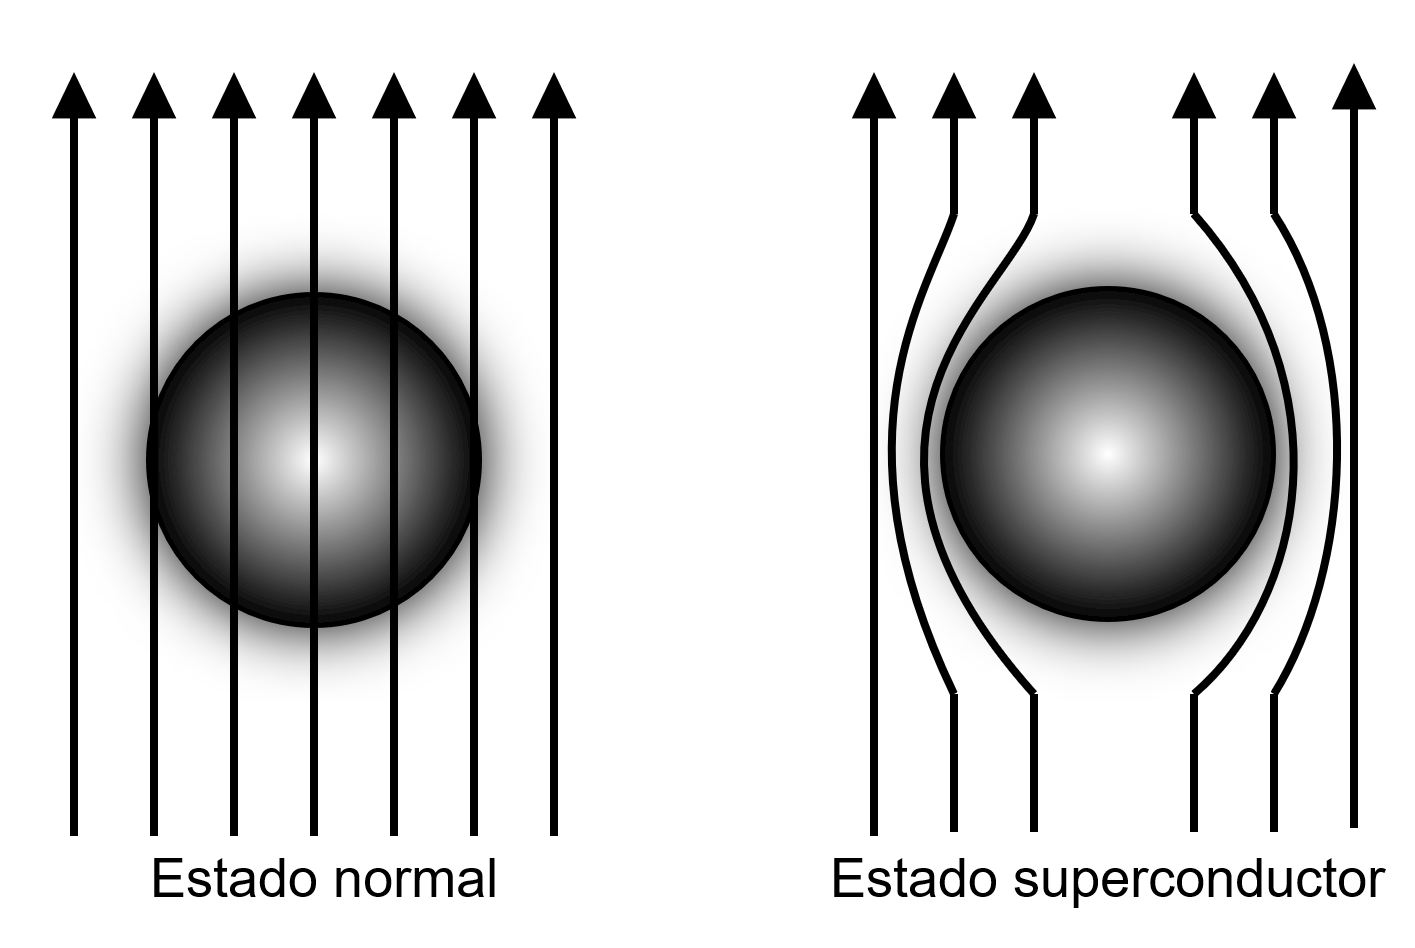
\includegraphics[width=0.6\textwidth]{gfx/superconductingsphere.png}
	\caption{Esfera de plomo en el seno de un campo magnético. A la izquierda por encima de la temperatura crítica. A la derecha el campo magnético es expulsado del interior de la esfera.}
	\label{fig:1}
\end{figure}

Esta explicación del esfecto Meissner recae en la suposición de que el campo magnético no es muy fuerte. Sea $\mc V$ el volumen de la esfera de plomo en fig. \ref{fig:1}. Si hacemos $\phi=0$ en toda la esfera, entonces el campo magnético puede penetrar libremente y de acuerdo a la ecuación \eqref{eq:1}, la energía es $\lambda m^4\mc V/8$. Si hacemos $\phi=m$, el campo es expedido del material y de acuerdo al funcional de energía, esto tiene un costo energético de aproximadamente $|B|^2\mc V/2$. El efecto Meissner ocurrirá si es favorecido energéticamente, esto pasa cuando la energía para expedir el campo magnético es menor a la energía para hacer $\phi=0$. Esto pasa cuando $B$ es menor a un valor crítico $B_{c}=\lambda^{1/2}m^2/2$. Este valor crítico es típicamente del orden de 10000 veces el campo magnético de la Tierra y está cerca de los imanes más potentes actualmente.

Ya que la energía para expedir al campo magnético es proporcional a $|B|^2$, la energía crece cuando $B$ aumenta. Como resultado de esto, un superconductor es repelido de una región donde el campo magnético es grande. Esto lleva al fenómeno de la levitación magnética (fig. \ref{fig:2}).

\begin{figure}[ht]
	\centering
	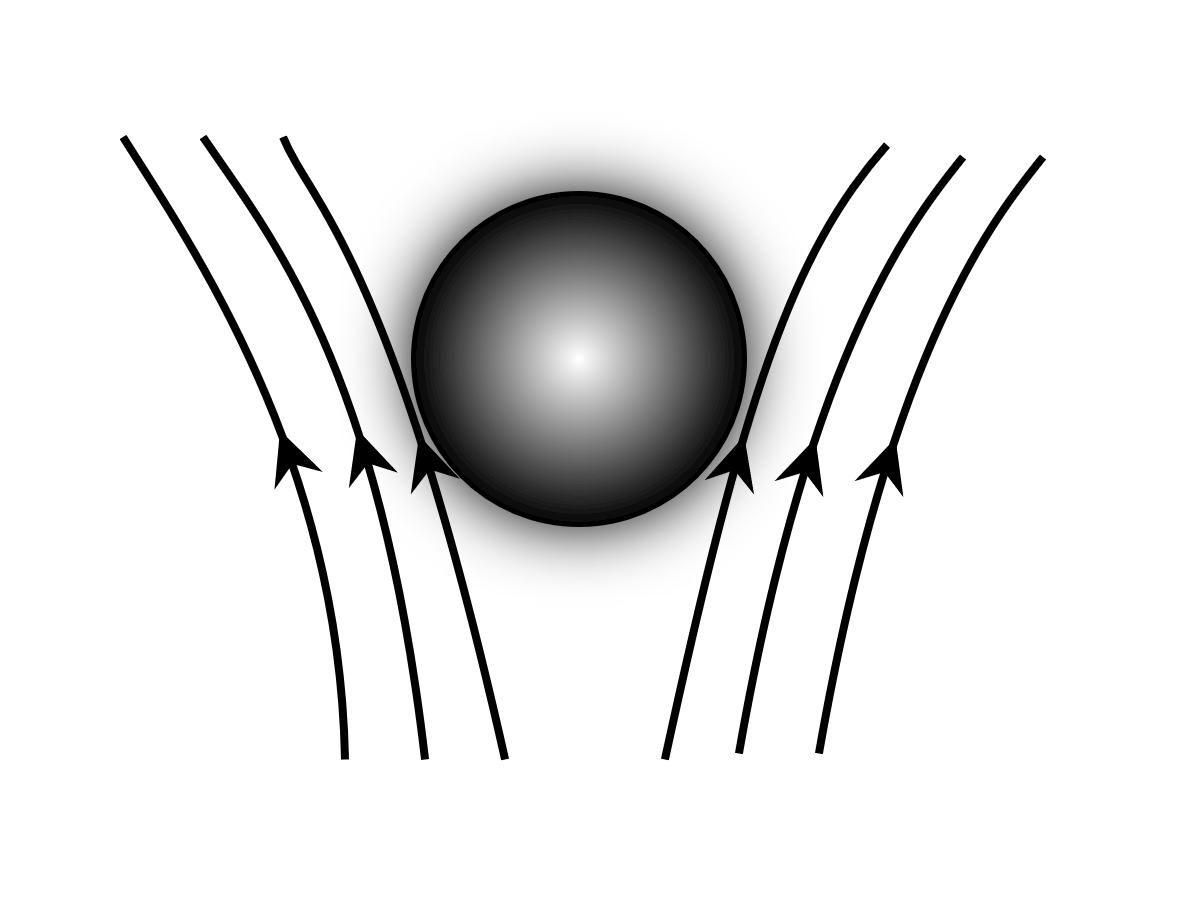
\includegraphics[width=0.6\textwidth]{gfx/maglev.png}
	\caption{Esfera superconductora es repelida de una región donde el campo magnético es fuerte.}
	\label{fig:2}
\end{figure}

Un material superconductor presenta corrientes eléctricas que fluyen en su interior y que son los responsables de cambiar la configuración del campo externo mostrado en fig. \ref{fig:2}. Las corrientes dentro del superconductor crean un campo magnético tal que la suma del campo externo con este campo interno se anula. Estas corrientes fluyen indefinidamente, ya que el efecto Meissner es energéticamente favorable. El hecho de que estas corrientes fluyan indefinidamente sin gasto energético es lo que conocemos como superconductividad.

Las ecuaciones de Maxwell independientes del tiempo demandan de que si el campo magnético es nulo en el interior de un superconductor, entonces la densidad de corrientes $\vec J$ también. Por lo tanto, las corrientes deben fluir en la superficie del material.

\subsection{Líneas de flujo}

Una línea de flujo es una región unidimensional dentro del superconductor donde la sección $\phi=0$. Estas líneas de flujo son de gran importancia científica y tecnológica y son conocidas como líneas de flujo de Abrikosov-Gorkov. Una representación de estas líneas de flujo en una esfera superconductora se muestra en figura \ref{fig:3}

\begin{figure}[ht]
	\centering
	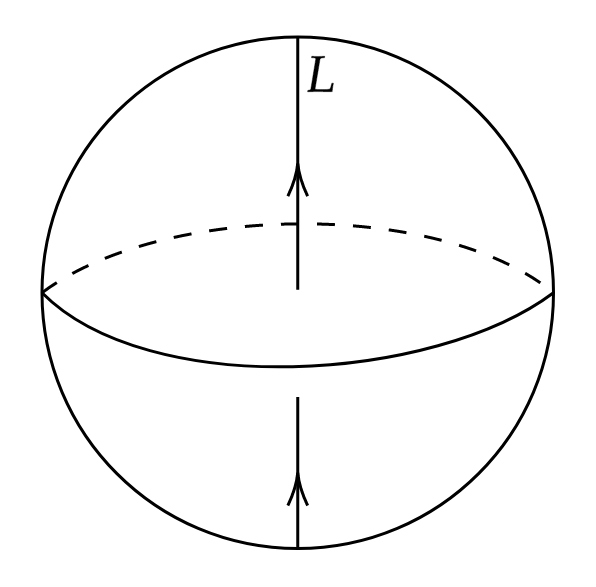
\includegraphics[width=0.5\textwidth]{gfx/fluxline.png}
	\caption{Linea de flujo dentro de una esfera superconductora. A lo largo de la línea $\phi=0$.}
	\label{fig:3}
\end{figure}

Podemos describir matemáticamente a las líneas de flujo como mínimos de un funcional de energía adecuado. En el modelo de Ginzburg-Landau, la función de energía es la suma de la energía para $\phi$, dada en \eqref{eq:1}, y la energía magnética, que es la integral de $|B|^2/2$. La función a minimizar es
\begin{align}
	V(\phi,B) = \int_{\m R^3}d^3x\bp{\f{|B|^2}2+\f 12|d_A\phi|^2+\f{\lambda}{8}(m^2-\phi^2)^2}.
\end{align}
Las ecuaciones de Euler-Lagrange nos devuelven las ecuaciones de la teoría de Ginzburg-Landau:
\begin{align}
	D_\mu D^\mu\phi+\f{\lambda}4\phi(m^2-\phi^2) &=0\\
	\eps_{ij}B_i+ie(\bar\phi D_j\phi-\phi\bar{D_i\phi}) &=0
\end{align}
Estas ecuaciones en derivadas parciales se pueden reducir a ecuaciones diferenciales ordinarias usando argumentos de simetría (como veremos en la sección \ref{sec:1.3}) en $\m R^2$. Soluciones a estas ecuaciones con el típico comportamiento $|\phi|\ra m$ y $d_A\phi\ra 0$ en el infinito son caracterizadas por un entero $n$, conocido como la primera clase de Chern. Soluciones existen, pero no se pueden escribir en una forma explícita, incluso la solución más básica de la línea vorticial de Abrikosov-Gorkov con $n=1$.

\subsection{Superconductores Tipo I y Tipo II}

Podemos reescalear la energía de Ginzburg-Landau de modo que sólo dependa de una constante adimensional. Considere los siguientes reescaleos: la sección $\phi$ puede ser reescaleada como $\phi\ra\phi/a$, las nuevas coordenadas espaciales $x\ra emx$, la conexión $A\ra eA$ y la curvatura $F\ra eF$. Con estas definiciones la constante de acoplamiento se vuelve adimensional $\lambda\ra\lambda/e^2$.

Una transición de fase ocurre cuando $\lambda=1$. Considere una superconductor que llena todo el espacio $\m R^3$ que posee líneas de flujo. Para $\lambda<1$, las líneas de flujo se atraen y se combinan para formar una sólo línea de flujo. Estos materiales son llamadas superconductores tipo I; ejemplos incluyen muchos metales puros. Para $\lambda>1$, las líneas de flujo se repelen. Un material con esta propiedad es llamado un superconductor tipo II.

La distinción de estos dos tipos de superconductores es de gran importancia práctica. Cuando un campo magnético externo se comienza a acercar al campo magnético crítico, líneas de flujo comienzan a penetrar el material. En superconductores Tipo I, estas líneas se atraen, provocando una región no superconductora (líneas de flujo la atraviesan) que va creciendo conforme seguimos aumentando el campo; eventualmente, la superconductividad se pierde. En el caso de superconductores Tipo II, las líneas de flujo se repelen, pudiendo formar un arreglo estable (fig. \ref{fig:4}). Como resultado, un superconductor Tipo II puede mantener su superconductividad incluso para campos magnéticos por encima del valor crítico, haciéndolos más útiles para aplicaciones tecnológicas.  Aún así, llegado a un segundo valor crítico del campo magnético, la superconductividad se pierde.

\begin{figure}[ht]
	\centering
	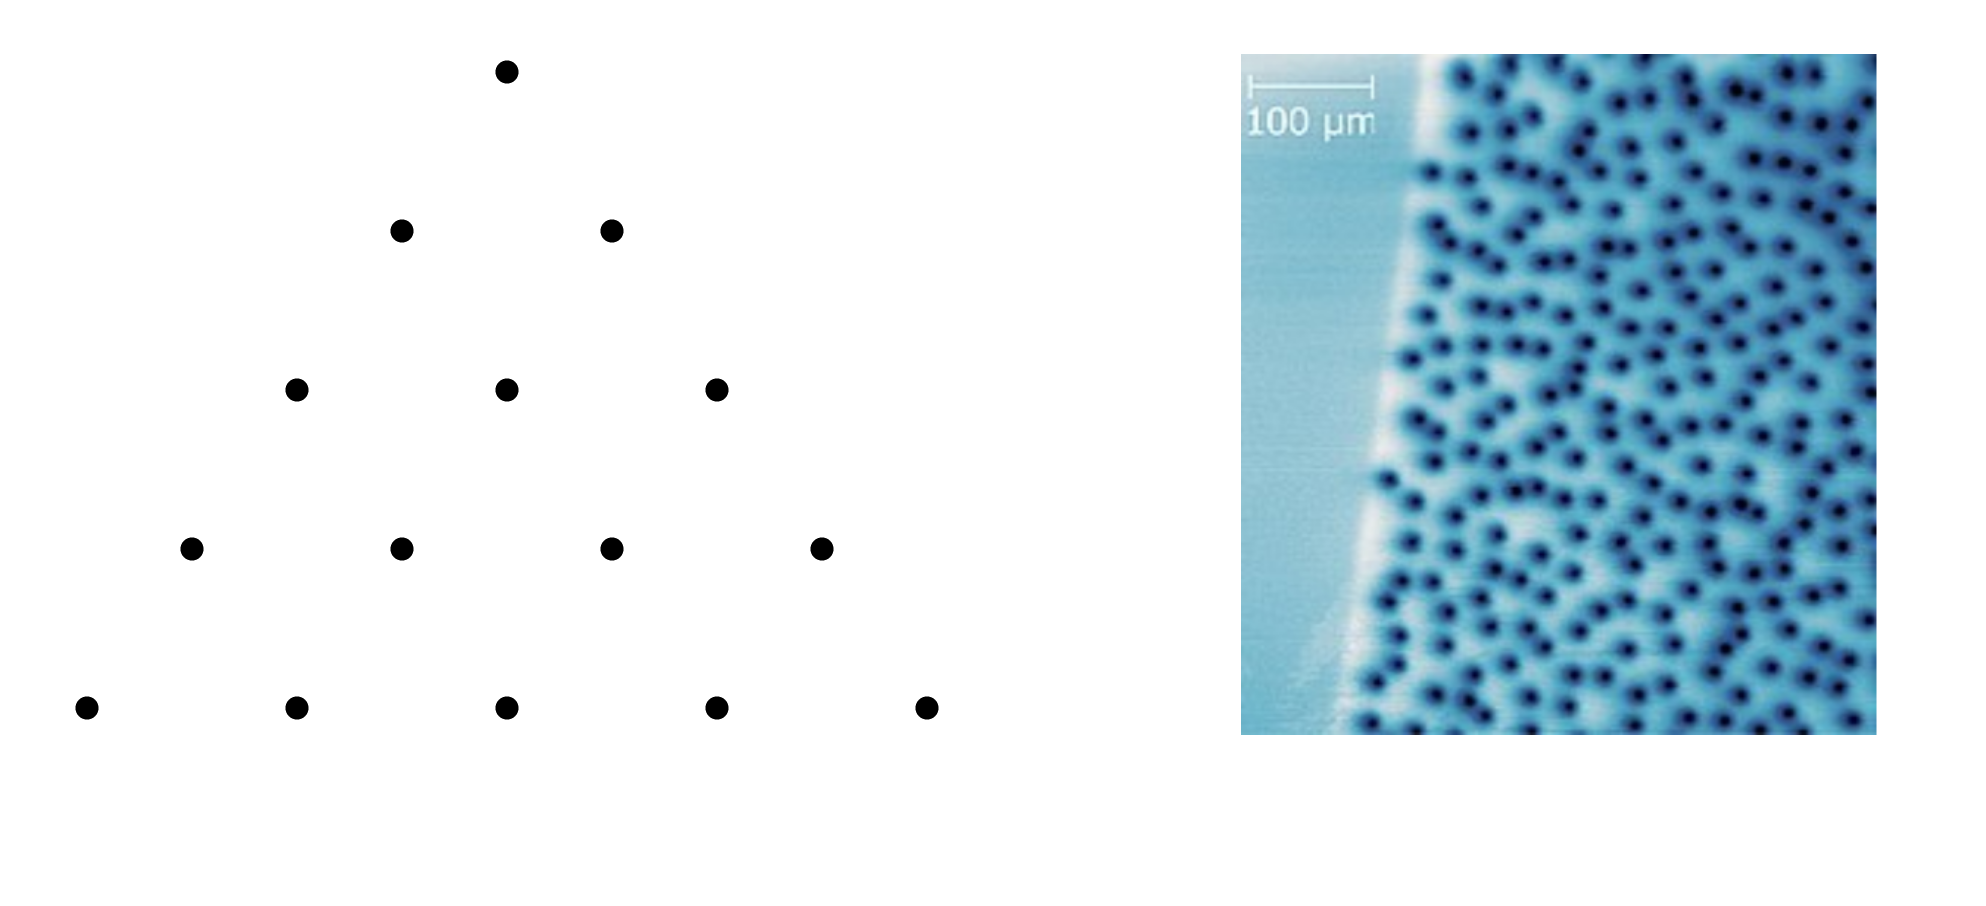
\includegraphics[width=0.6\textwidth]{gfx/type2superconductor.png}
	\caption{A la izquierda, un arreglo estable de líneas de flujo vistas desde arriba. A la derecha vórtices en una lámina delgada de 200 nm de YBCO, tomada usando microscopía SQUID.}
	\label{fig:4}
\end{figure}


\section{Modelo de Higgs abeliano}

El modelo de Higgs abeliano (o modelo de Maxwell-Higgs) es la versión relativista del modelo GL. La sección $\phi(x):\m R^{2+1}\ra\m C$ se le conoce ahora como campo de Higgs. Esta teoría es el paradigma para obtener soluciones vorticiales. La densidad lagrangiana de la teoría es
\begin{align}
    \mc L = -\f 14 F_{\mu\nu}F^{\mu\nu}+\f 12D_\mu\phi\overline{D^\mu\phi}-\f{\lambda}8(1-|\phi|^2)^2 \label{eq:2}
\end{align}
Este funcional corresponde a una teoría gauge pues el campo de Higgs se encuentra acoplado al campo electromagnético. La teoría tiene presenta las simetrías internas típicas del electromagnetismo, i.e., invarianza ante transformaciones de gauge $\phi\ra e^{i\al}\phi$ y $A_\mu\ra A_\mu-i\pr_\mu\al$. Las correspondientes ecuaciones de Euler-Lagrange son
\begin{align}
    D_\mu D^\mu\phi + \f{\lambda}2(1-|\phi|^2)\phi &=0,\label{eq:euler1}\\
    \pr_\mu F^{\mu\nu} &= J^\nu,\label{eq:euler2}
\end{align}
donde $J^\mu=\f i2(\bar\phi D^\mu\phi-\overline{D^\mu\phi}\phi)$ puede ser considerada como una \emph{corriente} generada por la simetría interna. Buscamos configuraciones de campos vorticiales, esto es, soluciones estáticas a $\eqref{eq:euler1}$ y $\eqref{eq:euler2}$ con energía finita. En el gauge temporal $A_0=0$, el funcional de energía de la configuración estática es
\begin{align}
    V_{\lambda} = \f 12\int_{\m R^2}\bp{B^2+D_i\phi\overline{D_i\phi}+\f{\lambda}4(1-|\phi|^2)^2}d^2x \label{eq:gl}
\end{align}
Podemos obtener la correspondiente teoría global haciendo $A_i=0$, obteniéndose
\begin{align}
    V_{\lambda} = \f 12\int_{\m R^2}\bp{|\nabla\phi|^2+\f{\lambda}4(m^2-|\phi|^2)^2}d^2x \label{eq:3a}
\end{align}
A esta teoría global se la conoce como teoría de Ginzburg-Landau global y sus soluciones son llamadas vortices globales. En este trabajo estamos especialmente interesados en el modelo de Higgs abeliano, sin embargo, analizaremos brevemente la teoría de Ginzburg-Landau global ya que algunos métodos nos servirán más tarde.

\section{Teoría de Ginzburg-Landau global}
\label{sec:1.3}

El funcional de energía $\eqref{eq:3a}$ es invariante ante rotaciones en el plano complejo $\phi\ra e^{i\al}\phi$ dónde $\al$ es una fase constante . Soluciones estáticas se obtendrán minimizando el funcional de energía, $\delta V_\lambda=0$, obteniéndose su ecuación de movimiento
\begin{align}
    \Delta\phi+\f{\lambda}2(m^2-|\phi|^2)\phi=0 \label{eq:3}
\end{align}
Dada esta simetría ante rotaciones en el plano complejo, resulta natural escribir el funcional de energía en términos de coordenadas polares $x^1=\rho\cos\theta$ y $x^2=\rho\sin\theta$
\begin{align}
    V_\lambda = \f 12\int_0^\infty\int_0^{2\pi}\bp{\pr_\rho\bar\phi\pr_\rho\phi+\f 1{\rho^2}\pr_\theta\bar\phi\pr_\theta\phi+\f\lambda 4(m^2-|\phi|^2)^2}\rho d\rho d\theta \label{eq:4}
\end{align}
Para que esta teoría presente solitones, sabemos\footnote{Ver Apéndice 1} que el campo de Higgs debe ser no trivial en el infinito y también $V_\lambda$ debe ser finita en el infinito. Observando la ecuación $\eqref{eq:4}$ vemos que para que el funcional sea finito en el infinito, $\rho\ra\infty$, se debe cumplir que el potencial cuártico y la derivada respecto al campo radial se anulen, esto pasa cuando
\begin{align}
    \lim_{\rho\ra\infty} |\phi| &= m \label{eq:5}\\
    \lim_{\rho\ra\infty} \pr_\rho\phi &= 0 \label{eq:6}
\end{align}
A partir de ahora, haremos un reescaleo de la teoría imponiendo $m=1$ sin pérdida de generalidad. Entonces, impondremos las condiciones de contorno $|\phi|\ra 1$ y $\pr_r\phi\ra 0$. La primera condición implica que $\phi_\infty = e^{i\chi(r,\theta)}$, mientras que la segunda condición implica que $\chi(r,\theta)=\chi(\theta)$. Otra propiedad que queremos que tenga el campo en el infinito es que sea univaluada, esto se traduce en que $\chi_\infty(2\pi)=\chi_\infty(0)+2\pi N$, donde $N\in\m Z$. Dado este comportamiento en el infinito, uno puede plantear el siguiente \emph{ansatz} para el campo de Higgs
\begin{align}
    \phi(\rho,\theta) = f_N(\rho)e^{iN\theta} \label{eq:7}
\end{align}
Donde $f_N(\rho)\xrightarrow{\rho\ra\infty} 1$ para satisfacer las condiciones de contorno.

El entero $N$ juega un papel muy importante en lo que veremos más adelante. En el contexto de la topología, $N$ es el llamado grado de un mapeo continuo. En el contexto de la física $N$ es llamado un número cuántico topológico.

Insertando el \emph{ansatz} $\eqref{eq:7}$ en la ecuación de movimiento $\eqref{eq:3}$ obtenemos una ecuación diferencial para $f_N(\rho)$
\begin{align}
    \f{d^2f_N}{d\rho^2}+\f 1\rho\f{d f_N}{d\rho}-\f{N^2}{\rho^2}f_N+\f{\lambda}2(1-f_N^2)f_N=0 \label{eq:8}
\end{align}
Soluciones de $\eqref{eq:8}$ existen para todo $N\neq 0$ [Manton,177] y se pueden encontrar numéricamente.

Esta teoría tiene un problema: la energía de las soluciones diverge logarítmicamente. Basta con ver el término del gradiente angular en $\eqref{eq:4}$ 
\begin{align}
    V_\lambda &= \pi\int_0^\infty\bp{f'^2_N(\rho)+\f{N^2}{\rho^2}f_N^2(\rho)}\rho d\rho \overset{\rho\ra\infty}{\sim} \pi N^2\int_0^\infty \f{d\rho}\rho\ra\infty \label{eq:9} 
\end{align}

\paragraph{Topología en la teoría global} Hemos visto que la densidad de energía decae a cero rápidamente cuando $|\vct x|\ra\infty$ si $|\phi|\ra 1$ y $\pr_\rho\phi\ra 0$ cuando $\rho\ra\infty$. Asumamos que estos límites existen. Entonces, $\phi_\infty(\theta)=e^{i\chi_\infty(\theta)}$, esto es, el campo en el infinito toma valores en la circunferencia $S^1_\infty$ y devuelve valores también en una circunferencia $S^1$. Interpretamos al campo como un mapeo $\phi_\infty:S^1_\infty\ra S^1$. El vacío tiene una topología no trivial, sin embargo, no hay configuraciones de campo con energía finita. Esto era debido a que la contribución a  la energía de la parte angular divergía logarítmicamente a menos que $N=0$.

\section{Vórtices en el Modelo Higgs abeliano}

Ahora, analicemos las soluciones vorticiales en el modelo de Higgs abeliano cuyo funcional de energía es $\eqref{eq:2}$. Este funcional es invariante gauge $\phi\ra e^{i\al(x)}\phi$ y $A_i\ra A_i+\pr_i\al$ y las respectivas ecuaciones de movimiento obtenidas de variar el funcional respecto a $\phi$ y a $A_i$ son
\begin{align}
    D_iD_i\phi+\frac{\lambda}{2}(1-|\phi|^2)\phi &= 0 \label{eq:11}\\
    \eps_{ij}\pr_jB+\frac{i}{2}(\bar\phi D_i\phi-\phi\overline{D_i\phi}) &= 0 \label{eq:12}
\end{align}
\paragraph{Un comentario sobre $\eqref{eq:12}$} Esta ecuación se puede interpretar como una versión bidimensional de la ecuación de Ampere. Podemos tratar a $J_i=\frac{i}{2}(\bar\phi D_i\phi-\phi\overline{D_i\phi})$ como una corriente en el plano.

Estamos interesados en configuraciones de campo que minimizen la energía y además que sea finita. Para esto imponemos las siguientes condiciones de contorno
\begin{align}
    \lim_{|\vct x|\ra\infty} |\phi| &= 1 \label{eq:13}\\
    \lim_{|\vct x|\ra\infty} B &= 0 \label{eq:14}\\
    \lim_{|\vct x|\ra\infty} D_i\phi &=0\label{eq:15}
\end{align}
Como en el caso de la teoría de Ginzburg-Landau global, condición $\eqref{eq:13}$ implica que $\phi_\infty(\vct x) = e^{i\chi_\infty(\vct x)}$, condición $\eqref{eq:14}$ requiere que $\vct A$ sea un gauge puro, es decir, $A_i=\pr_i\al(\vct x)$. Por último, condición $\eqref{eq:15}$ requiere que
\begin{align}
    im(\pr_i\chi_\infty-\pr_i\al)e^{i\chi_\infty} =0
\end{align}
de modo que $\pr_i(\chi_\infty-\al)=0$ y $\al=\chi_\infty+\text{cte.}$ Por lo tanto, la configuración de campo en el infinito es
\begin{align}
    \phi_\infty = e^{i\chi_\infty} &,\ \ A_i = \pr_i\chi_\infty \label{eq:16}
\end{align}
Tenemos la libertad de elegir el gauge $\chi_\infty=0$, obteniendo la siguiente configuración en el infinito $(\phi,A) = (1,0)$.

Queremos escribir a $\eqref{eq:2}$ en coordenadas polares, para esto definimos $A_\rho = A_1\cos\theta+A_2\sin\theta$ y $A_\theta=-A_1\rho\sin\theta+A_2\rho\cos\theta$, entonces
\begin{align}
    V_\lambda = \f 12\int_0^\infty\int_0^{2\pi}\bp{\f{1}{\rho^2}f_{\rho\theta}^2+\overline{D_\rho\phi}D_\rho\phi+\f 1{\rho^2}\overline{D_\theta\phi}D_\theta\phi+\f{\lambda}4(1-|\phi|^2)^2}\rho d\rho d\theta .\label{eq:17}  
\end{align}
Donde $f_{\rho\theta}=\pr_\rho A_\theta-\pr_\theta A_\rho=\rho B$, $D_\rho\phi=\pr_\rho\phi-iA_\rho\phi$ y $D_\theta\phi=\pr_\theta \phi-iA_\theta\phi$. Condición $\eqref{eq:14}$ implica que $A_\rho=\pr_\theta\al(\rho,\theta)$ y $A_\theta=\pr_\rho \al(\rho,\theta)$. Esto nos permite escribir un \emph{ansatz} para la configuración de campos
\begin{align}
    \phi(\rho,\theta) = f_N(\rho)e^{iN\theta},\ \ A_\theta(\rho,\theta) = N\al_N(\rho) \label{eq:18} 
\end{align}
donde $f_N\xrightarrow{\rho\ra\infty} 1$ y $\al_N\xrightarrow{\rho\ra\infty} 0$ para satisfacer las condiciones de contorno en el infinito. Insertando $\eqref{eq:18}$ en las ecuaciones de movimiento $\eqref{eq:11}$ y $\eqref{eq:12}$ obtenemos ecuaciones diferenciales para $f_N$ y $\al_N$:
\begin{align}
    \f{d^2f_N}{d\rho^2}+\f{1}{\rho}\f{df_N}{d\rho}-\f{1}{\rho^2}(N-\al_N)^2 f_N+\f{\lambda}2(1-f_N^2)f_N &=0\\
    \f{d^2\al_N}{d\rho^2}-\f{1}\rho\f{d\al_N}{d\rho}+(N-\al_N)f_N^2 &= 0
\end{align}
Se han demostrado en [Manton,333,50] que soluciones que satisfacen las condiciones de contorno existen para todo $N\neq 0$ y todo $\lambda>0$. Soluciones numéricas fueron obtenidas utilizando el lenguaje de programación Python, las cuales se muestran en el Apendice.

\paragraph{Carga topológica} El grado topológico del campo $\phi$ es la carga topológica del vórtice o también llamado primer número de Chern, definido como
\begin{align}
    c_1 = \f{1}{2\pi}\int_{\m R^2} f \label{eq:22}
\end{align}
donde $f=dA$ y $A$ es el campo de gauge escrito como una 1-forma. Entonces, el primer número de Chern es el flujo de campo magnético total. Se demuestra en [Manton] que $c_1$ es un entero\footnote{En general, el primer número de Chern no necesita ser un entero. Usando el teorema de Stokes en $\eqref{eq:22}$ podemos escribirla como una integral de línea a lo largo de un disco con radio muy grande $D_R$
\begin{align}
    c_1 = \lim_{R\ra\infty} \f 1{2\pi}\int_{D_R} A = \lim_{R\ra\infty}\int_0^{2\pi} A_\theta d\theta
\end{align}
Las condiciones de contorno sobre $A$ hacen que en el infinito se comporte como un gauge puro $A=d\al_\infty$. En particular, $A_\theta=\pr_\theta\al_\infty$ en el infinito, Por lo tanto,
\begin{align}
    c_1 = \f 1{2\pi}\int_0^{2\pi}\f{\pr\al_\infty}{\pr\theta}d\theta = \f 1{2\pi}(\al_\infty(2\pi)-\al_\infty(0))
\end{align}
En el caso de vórtices, las condiciones extras de contorno hacían que el campo fuera univaluado y por eso $\al_\infty(2\pi)-\al_\infty(0)=2\pi N$. Pero este no es el caso  general.}. En componentes y usando nuestra notación tenemos que
\begin{align}
    N = \f{1}{2\pi}\int_{\m R^2}d^2x B
\end{align}

\section{Vórtices críticos}

En esta sección vamos a ver que para un valor específico de la constante de acoplamiento $\lambda$, las ecuaciones de movimiento de segundo orden $\eqref{eq:11}$ y $\eqref{eq:12}$, se reducen a ecuaciones de primer orden, llamadas ecuaciones de Bogomolny.

\subsection{Cálculo de Bogomolny}

Analizaremos el cálculo clásico de Bogomolny [Bogomolny] de completar cuadrados en el funcional. Consideremos el funcional de GL para el modelo de Higgs abeliano $\eqref{eq:2}$. Este se puede escribir de la siguiente forma
\begin{align}
    V_\lambda = \f 12\int_{\m R^2}\bb{\bp{B-\f{\sqrt\lambda}2(1-|\phi|^2)}^2+B\sqrt\lambda(1-|\phi|^2)+|D_1\phi+iD_2\phi|^2}d^2x, \label{eq:1.5.1}
\end{align}
donde $|D_i\phi+iD_2\phi|^2=|D_1\phi|^2+|D_2\phi|^2+2(\pr_1\phi A_2-\pr_2\phi A_1)\phi$, que tambén se escribe, en el lenguaje de la geometría diferencial, como $|D_i\phi+iD_2\phi|^2=|D_1\phi|^2+|D_2\phi|^2+2\phi d\phi\wedge A$. Ahora analicemos el segundo término en $\eqref{eq:1.5.1}$:
\begin{align}
    \nonumber
    \int_{\m R^2} B\sqrt{\lambda}(1-|\phi|^2) d^2x &= \int_{\m R^2} B\sqrt{\lambda} d^2x-\int_{\m R^2}B\sqrt{\lambda}|\phi|^2 dx^2
\end{align}
\begin{align}
    \nonumber
    &= 2\pi N\sqrt{\lambda}-\sqrt{\lambda}\int_{\m R^2} |\phi|^2 dA \\ \nonumber
    &= 2\pi N\sqrt\lambda-2\sqrt{\lambda}\int_{\m R^2} d|\phi|^2\wedge A\\
    &= 2\pi N\sqrt\lambda-2\sqrt{\lambda}\int_{\m R^2} \phi d\phi\wedge A \label{eq:1.5.2}
\end{align}
 Vemos que el segundo término de $\eqref{eq:1.5.2}$ elimina exactamente al término producto de $|D_1\phi+iD_2\phi|$ sólo cuando $\lambda=1$. En ese caso, el funcional se escribe como
 \begin{align}
     V_{\lambda=1} = \f 12\int_{\m R^2}\bb{\bp{B-\f{1}2(1-|\phi|^2)}^2+|D_1\phi+iD_2\phi|^2}d^2x+ \pi N \label{eq:1.5.3}
 \end{align}
 
 \subsection{Desigualdad de Bogomolny}
 
 Los integrandos de $\eqref{eq:1.5.3}$ son no negativos por lo que la integral es necesariamente no negativa. Entonces, la siguiente desigualdad es evidente
 \begin{align}
     V_{\lambda=1}\geq \pi N\label{eq:1.5.2.1}
 \end{align}
 Ecuación $\eqref{eq:1.5.2.1}$ es conocida como desigualdad de Bogomolny.
 
 \subsection{Ecuaciones de Bogomolny}
 
 El caso interesante es cuando la desigualdad de Bogomolny se satura, i.e., $V_{\lambda=1}=\pi N$. Esto pasa cuando los integrandos de $\eqref{eq:1.5.3}$ se anulan por separado
 \begin{align}
     \left\{\begin{array}{c}
          D_1\phi+iD_2\phi = 0  \\
          B = \f 12(1-|\phi|^2)
     \end{array}\right. \label{eq:1.5.3.1}
 \end{align}
 Estas son conocidas como las ecuaciones de Bogomolny, y como se observa, son ecuaciones diferenciales de primer orden.
 
 Configuaraciones de campo que satisfacen las ecuaciones de Bogomolny $\eqref{eq:1.5.3.1}$  necesariamente satisfacen también las ecuaciones de movimiento $\eqref{eq:11}$ y $\eqref{eq:12}$ y, por lo tanto, son mínimos de la energía.
 
 Estas ecuaciones fueron derivadas por primera vez por Bogomolny en [Bogomolny,gab] utilizando este método de factorización. Esta propiedad de reducción de las ecuaciones de movimiento de segundo orden $\eqref{eq:euler1}$ y $\eqref{eq:euler2}$ a ecuaciones de primero orden se ha encontrado en muchos modelo en teorías de gauge. Uno de los primeros casos se encontró en la teoría de gauge no abeliana de Yang-Mills puro [Jaffe,Taubes]. En este caso, los solitones son llamados \emph{instantones} y corresponden a campos de gauge autoduales.
 Otra de las teorías de gauge en que podemos hacer un procedimiento de factorización es la teoría de Chern-Simons.
 
 Taubes, en [Manton,396,397], realizó un estudio sobre las ecuaciones de Bogomolny y obtuvo resultados importantes concernientes a vortices críticos. Estos resultados son presentados en el libro [Jaffe,Taubes]. Uno de estos resultados es el ahora conocido como Teorema de Taubes, el cuál analizaremos los aspectos más importantes en un capítulo posterior. Otro de los resultados importantes fue la reducción de las ecuaciones de Bogomolny a una ecuación escalar conocida como ecuación de Taubes. Esta ecuación fue generalizada por [Manton,Five vortex equations], obteniendo cinco ecuaciones vorticiales con soluciones analíticas conocidas.
 
 
 
 % Capítulo 1
% Chapter 2

\chapter{Cinco ecuaciones vorticiales} % Chapter title

\label{ch:taubes} % For referencing the chapter elsewhere, use \autoref{ch:examples} 

%----------------------------------------------------------------------------------------

En este capítulo enunciaremos el Teorema de Taubes y mostraremos los pasos más importantes para su demostración. Este teorema aparece por primera vez en [Taubes, N vortex]. El teorema muestra que un conjunto no ordenado de puntos en el plano complejo (no necesariamente distintos) determina únicamente una solución analítica de las ecuaciones de Bogomolny, también se demuestra que esta es la única solución $C^\infty$. La importancia del teorema es clara, sin embargo, no provee con una solución explícita de las ecuaciones de Bogomolny en el plano. Además de presentar este teorema, en la presente sección, mostraremos cinco ecuaciones vorticiales que dan soluciones explícitas en superficies de Riemann. 

\section{Teoremas de Taubes}
\label{sec:2.1}

Los teoremas de Taubes proveen una descripción de los espacios de módulo de soluciones de las ecuaciones de Bogomolny. El espacio de módulos de las solciones no es más que el espacio de soluciones módulo transformaciones de gauge. El primer teorema de Taubes es el siguiente:

\teo{Taubes 1}{Dado un entero $N\geq 0$ y un conjunto de puntos $\{Z_i\}, i=1,2,\cds k$ en el plano complejo $\m C$ con multiplicidades $d_1,d_2,\cds,d_k$, tal que $\sum d_j=N$, existe una solución de las ecuaciones de Bogomolny que es única a menos de una transformación de gauge, con las siguientes propiedades:
\begin{enumerate}
    \item La solución el globalmente $C^\infty$.
    \item Los ceros de $\phi$ son el conjunto de puntos $\{Z_i\}$. Además, cerca de sus ceros el campo se comporta como
    \begin{align}
        \phi\sim c_j(z-Z_j)^{n_j}, \ \ \ c_j\neq 0, \label{eq:2.1.0.1}
    \end{align}
    donde $n_j$ es la multiplicidad de $Z_j$.
\end{enumerate}}

Una de las consecuencias es que el número de vórtice es igual a $N$. Llamamos a esta solución una solución $N$-vorticial. Nótese que el teorema se puede usar, de forma totalmente análoga, para $N<0$ ya que una solución anti-vorticial corresponde a tomar la conjugada compleja de una solución vorticial.

Es fácil ver que para $N=0$, la solución es equivalente a la solución trivial $A_z=0$ y $\phi=1$.

\teo{Taubes 2}{Cualquier solución de las ecuaciones de Euler-Lagrange para $N>0$ y $\lambda=1$ es equivalente a una solución $N$-vorticial de las ecuaciones de Bogomolny.}

Una consecuencia de este teorema es que soluciones vorticiales del modelo abeliano de Higgs son $N$-vórtices o $N$-antivorticiales, es decir, no existes soluciones vórtice-antivórtice. Esto significa que, físicamente, las soluciones de las ecuaciones de Bogomolny son estables y su energía es la mínima.

\subsection{Espacio de módulos}

El espacio de módulos para las soluciones de las ecuaciones vorticiales está implícito en el primer teorema de Taubes. La descripción de una solución $N$-vorticial está descrita enteramente por $N$ puntos en el plano complejo, por lo que podemos argumentar que $\mc M=\m C^N$. Los puntos del plano pueden ser elegidos sin ningún orden en especial, por lo que para no contar $d_k$ veces un punto, debemos cocientar $\mc M$ por el grupo simétrico $S_N$. Entonces, $\mc M=\m C^N/S^N=\m C^N$.

\section{Estructura compleja de las ecuaciones de Bogomolny}
\label{sec:2.2}

En esta sección veremos como las ecuaciones de Bogomolny esconden una estructura compleja que será de gran ayuda en \ref{sec: 2.3}.

Consideremos la primera ecuación en $\eqref{eq:1.5.3.1}$ y desarrollemosla:
\begin{align}
    D_1\phi+iD_2\phi &= (\pr_1+i\pr_2)\phi-i(A_1+iA_2)\phi=0.\label{eq:2.2.0.1}
\end{align}
Definimos la derivada compleja $\pr_{\overline z}$ y el campo de gauge complejo $A_{\overline z}$ como
\begin{align*}
    \pr_{\overline z} &= \f 12(\pr_1+i\pr_2),\\
    A_{\overline z} &= \f 12(A_1+iA_2).
\end{align*}
Combinamos ambos en la derivada covariante compleja, definida como, $D_{\overline z} = \pr_{\overline z}-iA_{\overline z}$. Entonces, la primera ecuación de Bogomolny se escribe en forma compacta como
\begin{align}
    D_{\overline z}\phi =0. \label{eq:2.2.0.2}
\end{align}
Ecuación $\eqref{eq:2.2.0.2}$ guarda una semejanza con la versión compleja de las ecuaciones de Cauchy-Riemann $\pr_{\overline z}f=0$. Entonces, podemos decir que la primera ecuación de Bogmolny es una versión covariante de las ecuaciones de Cauchy-Riemann, por lo que, dan a entender que $\phi$ es una función analítica en el sentido covariante. Esto es más claro si consideramos que existe una función $w(z,\bar z)$ tal que $\pr_{\overline z}(e^{-w}\phi)=0$. Para que esto se cumpla, $w$ debe satisfacer $\pr_{\overline z}w=iA_{\overline z}$. Entonces, la función compleja $f=e^{-w}\phi$ es una función analítica, por lo tanto, tiene ceros aislados. Estos ceros coinciden con los ceros de $\phi$ pues $e^{-w}$ es no nula en todo punto. Además, $f$ localmente tiene la forma
\begin{align*}
    f(z)\sim c_j(z-Z_j)^{n_j}, \ \ \ c_j\in\m C.
\end{align*}
De aquí podemos leer el comportamiento de $\phi$ cerca de sus ceros.

Pero, queda la pregunta de que si $\pr_{\bar z}w=iA_{\bar z}$ tiene solución. Ya que $\f{1}{u-z}$ es la función de Green del operador $\pr_{\bar z}$, la solución puede escribirse como
\begin{align}
    w(z) = \f{1}{2\pi i}\int_{|u-z|<\epsilon}\f{i A_{\bar z}(z,\bar z)}{u-z} du d\bar u \label{eq:2.2.0.3}
\end{align}

Debido a la ecuación $\eqref{eq:2.2.0.2}$, una vez que se obtiene una solución para $\phi$, el campo de gauge queda determinado
\begin{align}
    A_{z} = i\pr_{z}\log\bar\phi, \ \ A_{\overline z} = -i\pr_{\overline z}\log\phi \label{eq:2.2.0.4}
\end{align}

\section{Reducción a una ecuación escalar}
\label{sec: 2.3}

Queremos escribir la segunda ecuación de Bogomolny en forma compleja. Para esto, escribimos $A_1$ y $A_2$ en términos de $A_z$ y $A_{\overline z}$ y luego reemplazando en $B$, obteniéndose
\begin{align}
    B = 2i(\pr_z A_{\overline z}-\pr_{\overline z} A_z)\label{eq:2.3.0.1}
\end{align}
La forma de la segunda ecuación de Bogomolny no cambia, simplemente el campo magnético se escribe de otra forma. Para combinar ambas ecuaciones de Bogomolny en una sóla ecuación, usemos $\eqref{eq:2.2.0.4}$ en $\eqref{eq:2.3.0.1}$
\begin{align}
    B = -2i^2(\pr_z \pr_{\overline z}\log\phi-\pr_{\overline z}\pr_z\log\bar\phi) = 2\pr_z\pr_{\overline z}(\log\phi+\log\bar\phi) = 2\pr_z\pr_{\overline z}\log|\phi|^2. \label{eq:2.3.0.2}
\end{align}
Entonces, la segunda ecuación se Bogomolny se escribe
\begin{align}
    \pr_z\pr_{\overline z}\log|\phi|^2 = \f{1}2(1-|\phi|^2) \label{eq:2.3.0.3}
\end{align}
Si hacemos $|\phi|^2 = e^{2u}$ y notamos que $\Delta=4\pr_z\pr_{\overline z}$, entonces $\eqref{eq:2.3.0.3}$ se escribe como
\begin{align}
    -\Delta u+e^{2u}-1 =0 \label{eq:2.3.0.4}
\end{align}
Ecuación $\eqref{eq:2.3.0.4}$ está incompleta pues $u$ tiene una singularidad logarítmica en los ceros de $\phi$, en donde tiende a $-\infty$. Entonces, ecuación $\eqref{eq:2.3.0.4}$ debe suplementarse con funciones delta con soporte justamente en estos ceros,
\begin{align}
    -\Delta u+e^{2u}-1 =-4\pi\sum_{j=1}^N\delta(z-Z_j)\label{eq:2.3.0.5}
\end{align}
Ecuación $\eqref{eq:2.3.0.5}$ es conocida como la ecuación de Taubes. Hasta el momento de escribir este trabajo, no se conocen soluciones explícitas a esta ecuación en el espacio plano.

\section{Vórtices en superficies riemannianas}\label{sec2.4}

En la sección anterior introducimos la ecuación de Taubes que describe vórtices en el plano, además, mencionamos que no existen hasta la fecha soluciones analíticas en el plano. Entonces, es natural preguntarse si pueden existir soluciones analíticas en espacios curvos para la ecuación de Taubes. Tales vórtices, si existen, se llaman vórtices integrables.

Los objetos de estudio son un campo escalar $\phi$ y un campo de gauge $A$, que son una sección y una conexión en un fibrado $U(1)$ \footnote{Localmente, la sección se representa por una función compleja sobre $M_0$ y la conexión como una 1-forma real con componentes $A=A_1dx^1+A_2dx^2$.} sobre $M_0$ respectivamente. Aquí $M_0$ es una superficie de Riemann que puede ser compacta o no (pero con un borde en el infinito). En coordenadas complejas $z=x^1+ix^2$, la métrica en $M_0$ es
\begin{align}
    ds_0^2 = \Om_0((dx^1)^2+(dx^2)^2)=\Om_0 dzd\bar z, \label{2.4.0.1}
\end{align}
donde $\Om_0$ es un factor conforme que depende de las coordenadas. El campo de gauge tiene curvatura $F=dA$, o en componentes, $F_{12}=\pr_1 A_2-\pr_2 A_1$. El campo magnético físico es $B=\f{1}{\Om_0}F_{12}$. Con estas generalizaciones, las ecuaciones de Bogomolny se escriben
\begin{align}
    D_1\phi+iD_2\phi &= 0, \label{2.4.0.2}\\
    B &= \frac{\Om_0}{2}(1-|\phi|^2).\label{2.4.0.3}
\end{align}
Las ecuaciones de Taubes también se modifican y toman la siguiente forma
\begin{align}
    -\Delta u+\Om_0 e^{2u}-\Om_0 =0, \label{eq:2.4.0.4}
\end{align}
donde debemos tener en cuenta el comportamiento logarítmico de $u$ cerca los ceros de $\phi$
\begin{align}
    u\sim \log |z-Z|+\text{constante}. \label{eq:2.4.0.5}
\end{align}
De esta forma podemos ignorar las funciones delta de Dirac en $\eqref{eq:2.3.0.5}$. Las soluciones vorticiales no deberían tener más singularidades en $M_0$. Si $u$ tiene un máximo en $M_0$ el laplaciano de $u$ es negativo, además, debido a la ecuación $\eqref{eq:2.4.0.4}$, $u\leq 0$ en el máximo y por lo tanto también en todo punto, a causa del principio del máximo. Este argumento es válido sólo si $M_0$ es compacta. En el caso de que no lo sea debemos imponer la condición $|\phi|=1$ o $u=0$ en el borde.

Podemos generalizar aún más la ecuación $\eqref{eq:2.4.0.4}$ de la siguiente manera
\begin{align}
    -\Delta u+\Om_0(C_0-Ce^{2u}) =0, \label{eq:2.4.0.6}
\end{align}
donde $C_0$ y $C$ son constantes reales. Es claro, que uno puede reescalear estas constantes multiplicando por un factor que se puede absorber en el factor conforme. Entonces, sin pérdida de generalidad podemos hacer que $C_0$ y $C$ tomen tres valores estándar $-1,0$ o $1$. Esto hace que hayan nueve posibles combinaciones y, por lo tanto, nueve ecuaciones vorticiales.  De estas nueve ecuaciones sólo cinco tienen soluciones vorticiales.

El segundo y tercer términos de $\eqref{eq:2.4.0.6}$ describen al campo magnético, entonces, para que describa un campo magnético físico se debe cumplir que $-C_0+C e^{u}\geq 0$. Esto excluye cuatro casos: $C_0=0$ o $C_0=1$, combinados con $C=-1$ o $C=0$. Los cinco casos restantes se resumen en la siguiente cuadro
\begin{table}[ht]
    \centering
    \begin{tabular}{l|c|c}
        Vórtices & $C_0$ & C \\ \hline
        Vórtices hiperbólicos (Taubes) & -1 & -1\\
        Vórtices de Popov & 0 & 1\\
        Vórtices de Jackiw-Pi & 1 & 1\\
        Vórtices de Bradlow & -1 & 0\\
        Vórtices de Ambjorn-Olesen & -1 & 1\\ \hline
    \end{tabular}
    \caption{Ecuaciones vorticiales}
    \label{tab:vortex}
\end{table}

Los vórtices hiperbólicos fueron obtenidos por primera vez por Witten [witten77] mediante una reducción de dimensión de una toería de Yang-Mills $SU(2)$. La motivación inicial de Witten era obtener soluciones autoduales $F_{\mu\nu}=\bar F_{\mu\nu}$ que posean simetría ante rotaciones y transformaciones de gauge. Esto lo llevó a plantear un ansatz para el campo de gauge no abeliano $A_\mu^a$ que reducía la acción de Yang-Mills a la acción de Maxwell-Higgs pero en un espacio con métrica $g^{\mu\nu}=r^2\delta^{\mu\nu}$, es decir, un espacio con curvatura constante negativa $-1$, llamado el espacio hiperbólico $\m H^2$. Las ecuaciones de autodualidad correspondían a las ecuaciones de Bogomolny con $\Om_0=\f{1}{r^2}$. En $\m H^2$, la ecuación de Taubes se reducía a la ecuación de Liouville, cuya solución general es conocida y está caracterizada por una función analítica arbitraria $f:\m H^2\ra\m H^2$.

La ecuación de Popov [Popov] surgió de una forma completamente análoga a lo obtenido por Witten, pero para una teoría de Yang-Mills $SU(1,1)$. En vez de una espacio hiperbólico, las soluciones de Popov son integrables en una esfera, que tiene curvatura constante positiva $+1$. La solución está dada por funciones racionales en la esfera $R:\m S^2\ra\m S^2$ [Manton sobre Popov].

Los vórtices de Jackiw-Pi [Jackiw-Pi 1y2] aparecen en la teoría abeliana de Chern-Simons y son integrables en el plano o en un toro (condiciones de contorno periódicas en el plano).

Los vórtices de Bradlow fueron introducidos por primera vez en [Manton five] son integrables en $H^2$. Este caso es el caso límite de la ecuación de Taubes cuando $N$ alcanza el valor máximo permitido en una superficie compacta.

La ecuación de Ambjorn-Olesen apareció en [Manton five 13 y 14] en su estudio sobre inestabilidades de campos magnéticos fuertes en la teoría electrodébil.

Todas estas ecuaciones, conocidas como ecuaciones de vórtices exóticas, son integrables en dos dimensiones, pero todas en una superficie de Riemann distinta. Mirando al cuadro anterior uno puede ver una conexión entre el coeficiente $C_0$ y la curvatura de la superficie de Riemann en la que son integrables. Esta conexión es presentada por primera vez en [Manton five].


El funcional de energía correspondiente es análogo al del modelo abeliano de Higgs pero con coeficientes distintos:
\begin{align}
    V_{\lambda} = \f 12\int_{M_0}\bb{B^2-\f{2C}{\Om_0}D_i\phi\overline{D_i\phi}+\f{\lambda}4(-C_0+C|\phi|^2)^2}\Om_0 d^2x. \label{eq:2.4.0.7}
\end{align}
El argumento a la Bogomolny muestra que para $\lambda=1$ el funcional se puede escribir como
\begin{align}
    V_{\lambda=1} = \f 12\int_{M_0}\bb{\bp{B^2+\f 12(C_0-C|\phi|^2)}^2-\f{2C}{\Om_0}|D_1\phi+iD_2\phi|^2}\Om_0 d^2x-\pi C_0 N. \label{eq:2.4.0.8}
\end{align}
Si las ecuaciones de Bogomolny se satisfacen la energía es estacionaria y tiene el valor de $-\pi C_0 N$. En el caso de que $C\leq 0$, el integrando de $\eqref{eq:2.4.0.8}$ es positivo, por lo tanto, la energía es minimizada.

\section{Vórtices como métricas cónicas}

En [Manton,23], N. Manton sugiere considerar la métrica original $ds_0^2$ conformemente reescaleada con el cuadrado del campo de Higgs,
\begin{align}
    ds^2 = e^{2u}ds_0^2,\label{eq:2.5.0.1}
\end{align}
donde $|\phi|^2=e^{2u}$. Más tarde, esta métrica fue estudiada a detalle por Baptista [Manton,15], razón por la cuál, a partir de ahora la métrica \eqref{eq:2.5.0.1} será llamada métrica de Baptista. En palabras de Manton: \emph{$ds^2$ define una geometría intrínseca de una solución vorticial, y en ciertos casos, resulta más fácil describir y visualizar esta geometría intrínseca que estudiar por separado $ds_0^2$ y $e^{2u}$}.

La métrica de Baptista no es una métrica riemanniana regular pues se anula en los centros de los vórtices donde $|\phi|=0$. Una de las consecuencias del Teorema de Taubes es que $\phi$, por lo tanto $u$, tienen una forma asintótica cerca de estos centros dada por \eqref{eq:2.1.0.1}. Consideremos el caso más simple, $N=1$, entonces $e^{2u}\sim\mu|z|^2$, donde $\mu$ es una constante positiva. La métrica $ds_0^2$ se escribe alrededor del centro como $ds_0^2=\Om_0(0)dzd\bar z$ y por lo tanto, la métrica de Baptista se escribe como $\mu\Om_0(0)|z|^2dzd\bar z\sim r^2(dr^2+r^2d\theta^2)$ en coordenadas polares. Haciendo el cambio $\rho=\f 12 r^2$ y $\chi=2\theta$, la métrica de Baptista se escribe como la métrica plana en coordenadas polares $d\rho^2+\rho^2d\chi^2$, pero el nuevo ángulo polar va de $0$ a $4\pi$. Esto define una métrica cónica, con exceso $2\pi$.

Baptista derivó una relación simple entre la curvatura de la métrica original y la curvatura de la métrica de Baptista. Para la derivación de esta ecuación seguimos el procedimiento de Manton. Comenzamos con la fórmula de la curvatura gaussiana para la métrica original,
\begin{align}
    K_0 = -\f{1}{2\Om_0}\nabla^2\log\Om_0\label{2.5.0.2}
\end{align}
La métrica de Baptista, con factor conforme $\Om=e^{2u}\Om_0$, tiene curvatura gaussiana
\begin{align*}
    K = -\f{1}{2\Om}\nabla^2\log\Om = -\f{1}{2e^{2u}\Om_0}\nabla^2(2u+\log\Om_0),
\end{align*}
de modo que ambas curvaturas están relacionadas por 
\begin{align*}
    -\f{1}{\Om_0}\nabla^2u=-K_0+Ke^{2u}.
\end{align*}
Pero $u$ también satisface la ecuación de Taubes,
\begin{align*}
    -C_0+Ce^{2u}=-\f{1}{\Om_0}\nabla^2u=-K_0+Ke^{2u}.
\end{align*}
Multiplicando por $\Om_0$, llegamos a la ecuación de Baptista
\begin{align}
    (K_0-C_0)\Om_0=(K-C)\Om\label{eq:2.5.0.3}
\end{align}
Esta ecuación permite desvelar una simetría escondida de las soluciones vorticiales, a la que Baptista llama propiedad de transitividad, que permite construir soluciones vorticiales a partir de otras deformando la métrica. Para ver más explícitamente esta propiedad de superposición de soluciones vorticiales, sea $h$ una solución vorticial en la superficie de Riemann $\Sigma$ con número vorticial $N$, por lo tanto, satisface la ecuación de Taubes
\begin{align*}
    -\Delta h+\Om_0(C_0-Ce^{2u}) =0
\end{align*}
En $\Sigma$ definamos la métrica cónica \eqref{eq:2.5.0.1} con $\Om=e^{2u}\Om_0$. Sea $\bar h$ una solución vorticial con número vorticial $\bar N$ en $(\Sigma,\Om)$, por lo tanto, satisface la ecuación de Taubes con este factor conforme modificado
\begin{align*}
    \Delta\bar h+\Om(C-C_1e^{2\bar h}) =0
\end{align*}
Si sumamos ambas ecuaciones diferenciales encontramos que
\begin{align*}
    -\Delta(h+\bar h)+C(\Om-\Om_0 e^{2h})+\Om_0 C_0-\Om C_1 e^{2\bar h} &= 0\\
    -\Delta(h+\bar h)+\Om_0(C_0-C_1 e^{2(h+\bar h)}) &= 0
\end{align*}
 y que $e^{h+\bar h}$ tiene número vorticial $N+\bar N$. Entonces, la superposición de una solución vorticial con constantes $(C,C_1)$ en una superficie de Riemann con métrica reescaleada, con una solución vorticial con constantes $(C_0,C)$ produce una solución vorticial con constantes $(C_0,C_1)$ y con npumero vorticial igual a la suma de los números vorticiales de cada solución.
 
 Parafraseando el resultado anterior, si queremos obtener una solución vorticial con número de vórtice $N+\bar N$ en una superficie de Riemann $(\Sigma,\Om_0)$, podemos primero hallar una solución $N$-vorticial en $(\Sigma,\Om_0)$ y luego encontrar una solución $\bar N$-vorticial en $(\Sigma,e^{2u}\Om_0)$. Por supuesto, el procedimiento opuesto es posible. Este resultado es poderoso, ya que conociendo una solución $1$-vorticial en cualquier superficie, aplicando recursivamente esta regla, uno puede construir una solución $N$-vorticial.
 
 \subsection{Vórtices integrables} \label{sec:2.5.1}
 En esta sección analizaremos el caso en que la ecuación de Taubes \eqref{eq:2.4.0.4} es integrable, es decir, presenta soluciones analíticas, en el sentido de que se pueden escribir explícitamente. 
 
 Cuando la curvatura $K_0$ de la superficie de fondo $(M_0,\Om_0)$ es constante, con un valor tal que satisface la ecuación de Baptista \eqref{eq:2.5.0.3}, diremos que la ecuación de Taubes o los vórtices son integrables. Entonces, los vórtices son integrables cuando $K_0=C_0$. Además, la métrica de Baptista en la superficie $(M,\Om)$ tiene una curvatura $K=C$ lejos de las singularidades cónicas. En este caso de curvatura constante, el problema se reduce a resolver la ecuación de Liouville. Las soluciones de la ecuación se conocen y han sido bien estudiadas. Estas soluciones se escriben en términos de una función holomorfa $f$, y las singularidades cónicas corresponden a puntos de ramificación de $f$, donde la derivada se anula. Para algunos de los vórtices, esta construcción es bien conocida, por ejemplo, los vórtices hiperbólicos obtenidos por Witten discutidos en \ref{sec2.4}.
 
 La reducción a la ecuación de Liouville es la siguiente. Escribamos el factor conforme de la métrica de Baptista como $\Om=e^{2v}$. Entonces, usando la ecuación de curvatura gaussiana para $\Om$, esta se reduce a la ecuación de Liouville
 \begin{align}
	 \nabla^2 v=-Ce^{2v}, \label{eq:2.5.1.1}
 \end{align}
 donde reemplazamos $K=C$. La solución general de \eqref{eq:2.5.1.1} en una región simplemente conexa en el plano $z$ es
 \begin{align}
	 \Om = e^{2v} = \f{4}{(1+C|f(z)|^2)^2}\left|\f{df}{dz}\right|^2, \label{eq:2.5.1.2}
 \end{align}
 donde $f$ es una función holomorfa. Esta reducción también se puede hacer para la métrica de fondo, obteniéndose una expresión análoga a \eqref{eq:2.5.1.2}
 \begin{align}
	 \Om_0 = \f{4}{(1+C_0|z|^2)^2}. \label{eq:2.5.1.3}
 \end{align}
 Notemos que $|\phi|^2 = e^{2u}=\Om/\Om_0$, esto nos una expresión explícita para la solución a todos los casos integrables
 \begin{align}
	 |\phi|^2 = \f{(1+C_0|z|^2)^2}{(1+C|f(z)|^2)^2}\left|\f{df}{dz}\right|^2. \label{eq:2.5.1.4}
 \end{align}
 Uno puede elegir una gauge para el campo de Higgs y eliminar cualquier fase que pueda surgir para obtener
 \begin{align}
	 \phi = \f{1+C_0|z|^2}{1+C|f(z)|^2}\f{df}{dz}. \label{eq:2.5.1.5}
 \end{align}
En el caso particular de la ecuación de Taubes en el espacio hiperbólico tenemos $C_0=C=-1$ y $f$ es una función holomorfa del plano hiperbólico al plano hiperbólico $f:\m H^2\ra\m H^2$. En el modelo del disco de Poincaré, $f$ es una función racional de Blaschke
\begin{align}
	f(z) = \prod_{m=1}^{N+1}\f{z-a_m}{1-\bar a_m z} \label{eq:2.5.1.6}
\end{align}
 con $|a_m|<1$. El ejemplo más simple es cuando $a_m=0$, de modo que $f(z)=z^{N+1}$. Claramente, $\f{df}{dz}$ tiene $N$ ceros, lo que indica que hay $N$ vórtices. Todos estos vórtices son coincidentes en el origen y el campo de Higgs toma la forma
 \begin{align}
	 \phi = \f{(N+1)z^N(1-|z|^2)}{1-|z|^{2(N+1)}} \label{eq:2.5.1.7}
 \end{align}
 Nótese que se satisface $|\phi|\ra 1$ cuando nos acercamos al borde del disco de Poincaré $|z|\ra 1$. 
 
 Fórmulas similares se han hallado en la construcción de soluciones vorticiales para los vórtices de Popov con $C_0=C=1$. Estos vórtices viven en una esfera unitaria, y son construidos usando una función meromorfa $f$ de la esfera de Riemann a la esfera de Riemann. Tales funciones meromorfas deben ser racionales para asegurar la finitud del número de vórtice $N$:
 \begin{align}
	 f(z) = \f{p(z)}{q(z)}, \label{eq:2.5.1.8}
 \end{align}
 donde $p(z)$ y $q(z)$ son polinomios en $z$ sin raíces en común. Si ambos polinomios tienen grado $n$, entonces $\f{df}{dz}$ tiene $N=2n-2$ ceros. Nótese que los vórtices sólo pueden tener número vorticial par, sin embargo, es posible que existan soluciones con $N$ impar. % Capítulo 2
% Chapter 3

\chapter{Vórtices integrables a partir de autodualidad} % Chapter title

\label{ch:selfduality} % For referencing the chapter elsewhere, use \autoref{ch:mathtest}

%----------------------------------------------------------------------------------------

Contatto y Dunajski demostraron que las cinco soluciones vorticiales integrables obtenidas por Manton surgen como reducción de simetría de las ecuaciones de autodualidad de Yang-Mills en una cuatro variedad. En este capítulo introduciremos brevemente la teoría de Yang-Mills y las ecuaciones de (anti-)autodualidad , mostrando algunas de las soluciones instantónicas. Mostraremos explícitamente el cálculo hecho por Witten y obtendremos las soluciones vorticiales ya vistas en el plano hiperbólico. Luego, nos evocaremos a mostrar los resultados de Contatto y Dunajski, basándonos principalmente en [Contatto-Dunajski]

\section{Teoría de Yang-Mills}

Los instantones son solitones topológicos de la teoría de Yang-Mills pura definidas en un espacio euclídeo cuadrimensional. Consideraremos a los instantones como solitones estáticos en un espacio de cuatro dimensiones, de modo que son del mismo tipo que los vórtices que estuvimos estudiando.

La motivación para considerar un espacio euclídeo cuadrimensional y no el espacio tiempo de Minkowski $3+1$-dimensional es que en la Teoría Cuántica de Campos debemos calcular integrales de camino, las cuáles deben ser continuadas analíticamente (con una rotación de Wick) para estar bien definidas. Llamaremos al tiempo euclídeo $it$ como la coordenada $x^4$ en una teoría estática. La importancia de las soluciones clásicas es que proveen la contribución dominante a la integral de caminos, en particular, los instantones generan efectos cuánticos no perturbativos.

En el contexto más general de las teorías de Gauge, las teorías de Yang-Mills son ejemplos especiales de teorías de gauge con grupos de simetría no abelianos.

Consideremos una teoría de gauge $SU(2)$ con un potencial de gauge $A_\mu, \mu=1,\cdots,4$, tomando valores en el álgebra de Lie $\mf{su}(2)$. El tensor de campo asociado es
\begin{align}
	F_{\mu\nu} = \pr_\mu A_\nu-\pr_\nu A_\mu+[A_\mu,A_\nu] \label{eq:3.1.0.1}
\end{align}
La teoría de Yang-Mills pura está descrita por la siguiente acción
\begin{align}
	S=-\f 18\int d^4x \Tr(F_{\mu\nu}F_{\mu\nu}), \label{eq:3.1.0.2}
\end{align}
donde ahora usamos la métrica euclidiana es $(+,+,+,+)$. La variación de esta acción permite obtener la ecuación de campo de Yang-Mills \footnote{El cálculo explícito de la variación de la acción de Yang-Mills se muestra en el apéndice \ref{app:a1}}
\begin{align}
	D_\mu F_{\mu\nu} =0 \label{eq:3.1.0.3}
\end{align}
Introduzcamos la $2$-forma $F=\f 12F_{\mu\nu}dx^\mu\wedge dx^\nu$ que representa el campo electromagnético. En un espacio de cuatro dimensiones el dual de Hodge de una $2$-forma es otra dos forma. En componentes, el dual de Hodge de $F$, $\star F$, está definido como
\begin{align}
	\star F_{\mu\nu} = \f 12\eps_{\mu\nu\al\be}F_{\al\be},  \label{eq:3.1.0.4}
\end{align}
donde $\eps_{\mu\nu\al\be}$ es el tensor totalmente antisimétrico con la convención $\eps_{1234}=-1$. Usando el hecho de que $\Tr(F_{\mu\nu}F_{\mu\nu})=\Tr(\star F_{\mu\nu}\star F_{\mu\nu})$ \footnote{Demostración en Apéndice \ref{app:a2} }, la acción \eqref{eq:3.1.0.2} puede ser reescrita como
\begin{align}
	S = -\f 1{16}\int\bb{\Tr\bp{(F_{\mu\nu}\mp\star F_{\mu\nu})(F_{\mu\nu}\mp\star F_{\mu\nu})}\pm 2\Tr(F_{\mu\nu}\star F_{\mu\nu})}d^4x \label{eq:3.1.0.5}
\end{align}
Definamos la siguiente cantidad
\begin{align}
	N = -\f{1}{8\pi^2}\int\Tr(F_{\mu\nu}\star F_{\mu\nu})d^4x, \label{eq:3.1.0.6}
\end{align}
que no es más que el segundo número de Chern para un campo de gauge $SU(2)$ en $\m R^4$\footnote{Para una pequeña introducción, véase el Apéndice}. El primer término es un cuadrado, por lo que es no negativo. Esto conlleva a la siguiente desigualdad
\begin{align}
	S\geq\pi^2|N|, \label{eq:3.1.0.7}
\end{align}
que es análoga a la desigualdad de Bogomolny que derivamos para los vórtices. Estamos interesados con campos que hagan la acción finita, esto implica que $F_{\mu\nu}=0$ cuando $|x|\ra\infty$, esto implica que cuando $|x|\ra\infty$ el campo de gauge tiende a un gauge puro
\begin{align}
	A_\mu = -\pr_\mu g_{\infty}g_\infty^{-1} \label{eq:3.1.0.7}
\end{align}
para algún $g_\infty\in SU(2)$ definido en el infinito espacial. En este caso $N$ es un número entero y es igual al grado del mapeo $g_\infty: S_\infty^3\ra SU(2)$.

De la ecuación \eqref{eq:3.1.0.5} es inmediato que la desigualdad \eqref{eq:3.1.0.7} se satura cuando los campos son autoduales o anti autoduales
\begin{align}
	F_{\mu\nu} = \pm\star F_{\mu\nu}. \label{eq:3.1.0.8}
\end{align}
Estas son las ecuaciones de (anti)autodualidad de Yang-Mills. Soluciones de estas ecuaciones que hacen finita la acción son llamados (anti)instantones. $N$ es un entero positivo para campos autoduales no triviales y se interpreta como el número de instantones (análogamente $|N|$ es el número de anti instantones si $N<0$).

La solución general para el instantón con $N=1$ fue obtenida por primera vez por Belavin \emph{et al.} [Manton,47]. Más tarde, 't Hooft [Manton,402], obtuvo esta y otras soluciones multinstantónicas utilizando un ansatz. Para presentar el ansatz de 't Hooft, introduzcamos el tensor antisimétrico $\sg_{\mu\nu}$, definido como
\begin{align}
	\sg_{i4}=\tau_i, \ \ \ \sg_{ij}=\eps_{ijk}\tau_k, \ i,j=1,2,3 \label{eq:3.1.0.9}
\end{align}
y que tiene la propiedad de ser anti autodual: $\f{1}2\eps_{\mu\nu\al\be}\sg_{\al\be}=-\sg_{\mu\nu}$. El potencial de gauge autodual se contruye a partir de un campo escalar real $\rho$ como
\begin{align}
	A_\mu = \f{i}2\sg_{\mu\nu}\pr_\nu\log\rho \label{eq:3.1.0.10}
\end{align}
Si sustituimos este ansatz en \eqref{eq:3.1.0.8} llegamos a 
\begin{align}
	\f 1{\rho}\nabla^2\rho=0 \label{eq:3.1.0.11}
\end{align}
que no es más que la ecuación de Laplace en $\m R^4$. La solución instantónica con $N=1$ es generada por una solución que tiene un polo en un cuadrivector arbitrario constante $a\in\m R^4$
\begin{align}
	\rho(x) = 1+\f{\lambda^2}{|x-a|^2}. \label{eq:3.1.0.12}
\end{align}
La constante positiva $\lambda$ representa el ancho del instantón, en el sentido que la acción es máxima en $x=a$ y decae a la mitad cuando $|x-a|\leq\lambda$. Esta solución puede ser usada para generar instantones con $N$ arbitrario haciendo que la solución de la ecuación de Laplace tenga $N$ polos distintos
\begin{align}
	\rho(x) = 1+\sum_{j=1}^N\f{\lambda_j^2}{|x-a_j|^2},
\end{align}
con anchos y posiciones arbitrarias.

Este ansatz lleva a que el campo de gauge sea singular. Considere de nuevo la solución con $N=1$ con $a=0$, usando \eqref{eq:3.1.0.10} podemos ver que el potencial tiene una singularidad en $x=0$
\begin{align}
	A_\mu^{sing} = \f i2\sg_{\mu\nu}\f{-2\lambda^2x^\nu}{x^2(x^2+\lambda^2)}. \label{eq:3.1.0.13}
\end{align}
Sin embargo, mediante una transformación de gauge singular podemos remover la singularidad
\begin{align}
	A_\mu^{reg} = -i\sg_{\mu\nu}\f{x^\nu}{(x^2+\lambda^2)}. \label{eq:3.1.0.14}
\end{align}

\subsection{Espacio de módulos del instantón $SU(2)$}

Para especificar completamente el instantón \eqref{eq:3.1.0.12} hace falta conocer cinco parámetros reales, a saber, las cuatro componentes de $a$ y el ancho del instantón $\lambda$. Además de estos parámetros, se debe incluir una transformación de gauge $SU(2)$ para especificar la orientación del instantón. Esto agrega tres parámetros extra, teniendo un total de ocho. Por lo tanto, el espacio de módulos del instantón $N=1$, $\mc M_1$, tiene ocho dimensiones.

Resulta de mucho interés en matemática y física matemática estudiar estos espacios de módulos y sus métricas, en parte, debido a los trabajos de Donaldson y Witten sobre 4-variedades [Manton,111,112].  Para instantones en $\m R^4$ estos espacios de módulos son ejemplos de variedades hiperkähler. La métrica en el espacio de módulos se define restringiendo la métrica natural del espacio de configuraciones a la subvariedad de instantones. Atiyah, Hitchin y Singer [Manton,19] mostraron que el espacio de módulos para el instantón con carga $N$, $\mc M_N$, tiene dimensión $8N$. Cuando todos los instantones están muy separados entre ellos, los $8N$ parámetros pueden pensarse como $8$ parámetros para cada uno de los $N$ instantones.

\subsection{Solución multinstantónica de Witten}

Históricamente, la primera solución multinstantónica fue encontrada por Witten [Witten77] antes del descubrimiento de las soluciones de t' Hooft. Como se explicó en \ref{sec2.4} el enfoque de Witten fue encontrar instantones con simetría cilíndrica en cuatro dimensiones (simetría ante rotaciones alrededor del eje $x^4$). Explícitamente, el ansatz de Witten plantea el siguiente campo de gauge $SU(2)$
\begin{align} \label{eq:3.1.2.1}
	\begin{split}
	A_i^a &= \f{\phi_2+1}{r^2}\eps_{jak}x_k+\f{\phi_1}{r^3}[\delta_{ja}r^2-x_jx_a]+A_1\f{x_jx_a}{r^2},\\
	A_0^a &= \f{A_0x^a}r.
	\end{split}
\end{align}
donde los índices $j,k$ son índices espaciales y $a$ es índice de isoespín, es decir, indica el generador $t^a$ de $SU(2)$. Además, $\phi_1$, $\phi_2$, $A_0$ y $A_1$ son funciones de $x^4$ y $r$. Witten argumentó que este ansatz es el más general con simetría ante rotaciones y transformaciones de gauge. Usando \eqref{eq:3.1.2.1} uno puede calcular el tensor de campo $F_{\mu\nu}^a$ y su dual $\star F_{\mu\nu}^a$:
\begin{align}\label{eq:3.1.2.2}
	\begin{split}
	F_{0i}^a &= (\pr_4\phi_2-A_0\phi_1)\f{\eps_{iak}x_k}{r^2}+(\pr_4\phi_1+A_0\phi_2)\f{(\delta_{ai}r^2-x_a x_i)}{r^3}+r^2(\pr_4 A_1-\pr_1 A_0)\f{x_ax_i}{r^4},\\
	\f 12\eps_{ijk}F_{jk}^a &=-\f{\eps_{ias}x_s}{r^2}(\pr_1\phi_1+A_1\phi_2)+\f{(\delta_{ai}r^2-x_a x_i)}{r^3}(\pr_1\phi_2-A_1\phi_1)+\f{x_ax_i}{r^4}(1-\phi_1^2-\phi_2^2)
	\end{split}
\end{align}
donde $\pr_1=\pr/\pr_r$. La forma de \eqref{eq:3.1.2.2} sugiere que consideremos a $\phi=\phi_1+i\phi_2$ como un campo escalar complejo de Higgs interactuando con un campo de gauge bidimensional $A_\mu=(A_0,A_1)$, con derivada covariante $D_\mu\phi_i=\pr_\mu\phi_i+\eps_{ij}A_\mu\phi_j$. Insertando \eqref{eq:3.1.2.2} en la acción de Yang-Mills \eqref{eq:3.1.0.2} se tiene
\begin{align}
	S = \f{1}{8}\int d^3x\int dt F_{\mu\nu}^a F_{\mu\nu}^a = 8\pi\int_{-\infty}^{\infty}\int_0^\infty dr\bb{\f 12(D_\mu\phi_i)^2+\f{1}8r^2 F_{\mu\nu}^2+\f{1}4r^{-2}(1-|\phi|^2)^2}, \label{eq:3.1.2.3}
\end{align}
donde ahora $F_{\mu\nu}=\pr_\mu A_\nu-\pr_\nu A_\mu$. La acción de Yang-Mills se ha reducido a una versión modificada del funcional de energía del modelo abeliano de Higgs. De hecho, en un espacio curvo con métrica $g^{\mu\nu}$, el funcional de energía se puede escribir
\begin{align}
	\int d^2x\sqrt{g}\bb{\f 12g^{\mu\nu}D_\mu\phi_i D_\nu\phi_i+\f{1}8 g^{\mu\al}g^{\nu\be}F_{\mu\nu}F_{\al\be}+\f 14(1-|\phi|^2)}, \label{eq:3.1.2.4}
\end{align}
donde $g=\det g^{\mu\nu}$. Esta ecuación coincide con \eqref{eq:3.1.2.3} si $g^{\mu\nu}=r^2\delta^{\mu\nu}$. Esta métrica corresponde a un espacio con curvatura constante negativa igual a $-1$. Es decir, que $x^4$ y $r$ son coordenadas en un espacio hiperbólico $\m H^2$.

Si insertamos los tensores de campo \eqref{eq:3.1.2.2} en las ecuaciones de autodualidad, estas se reducen a las ecuaciones de Bogomolny para vórtices hiperbólicos discutidos en \ref{sec2.4} . Estas ecuaciones son
\begin{align}
	\begin{split}
	D_4\phi+iD_r\phi &=0,\\
	B-\f{1}{2r^2}(1-|\phi|^2) &=0,
	\end{split}
\end{align}
donde $B=\pr_4 A_1-\pr_r A_0$. Estas ecuaciones se resuelven derivando la ecuación de Taubes correspondiente y luego reduciéndola a la ecuación de Liouville. Esto lo hicimos explícitamente en \ref{sec:2.5.1}.


\section{Cinco ecuaciones vorticiales a partir de autodualidad}

En esta sección expondremos el trabajo de Conttato y Dunajski [ContDunaj] sobre la obtención de las cinco ecuaciones vorticiales a partir de reducciones de simetría de las ecuaciones de anti autodualidad de Yang-Mills en cuatro dimensiones.




%----------------------------------------------------------------------------------------

 % Capítulo 3
% Chapter X

\chapter{Chapter Title} % Chapter title

\label{ch:name} % For referencing the chapter elsewhere, use \autoref{ch:name} 

%----------------------------------------------------------------------------------------

\section{Section Title}

Content

%------------------------------------------------

\subsection{Subsection Title}

Content

%------------------------------------------------

\subsection{Subsection Title}

Content

%----------------------------------------------------------------------------------------

\section{Section Title}

Content % Capítulo 4

\cleardoublepage % Empty page before the start of the next part

%------------------------------------------------

\ctparttext{En esta parte vamos a analizar formas en que podemos modificar el modelo abeliano de Higgs para obtener nuevos comportamientos y tal vez nuevas soluciones analíticas.} % Text on the Part 2 page describing the content in Part 2

\part{Modelos modificados} % Second part of the thesis

% Chapter 5

\chapter{Modelos de Higgs abelianos modificados} % Chapter title

\label{ch:ahmmod} % For referencing the chapter elsewhere, use \autoref{ch:name} 

%----------------------------------------------------------------------------------------

La existencia y analiticidad de los vórtices abelianos en el plano fueron estudiados extensivamente por Taubes y Jaffe en [TaubesJaffe]. En capítulo 2 analizamos los resultados más importantes de estos papers. Modelos modificados han sido propuestos una multitud de veces, por ejemplo, Lohe [Lohe43] admite otros tipos de potenciales y modifica el término cinético del campo de modo que el truco de Bogomolny se pueda aplicar también. Veremos más adelante en este capítulo que esta condición es muy usada para constreñir la forma de los factores que modifican los términos cinéticos y el potencial.

En este capítulo vamos a presentar un modelo modificado propuesto por Contatto [Contatto2017] que admite vórtices estáticos. Contatto se vale de un análisis de ecuaciones diferenciales para hallar todos los posibles casos integrables de una familia de modelos modificados. A su vez, también se presenta una solución explícita.

Otra forma de modificar el modelo que exploraremos en este capítulo es agregar impurezas del tipo eléctrico y magnético. Tales impurezas fueron estudiadas por primera vez por Tong y Wong [TongWong2014] basándose en resultados parecidos en teorías supersimétricas en 2+1. Las cinco ecuaciones vorticiales que estudiamos en capítulo 2 son generalizadas por Gudnason y Ross en [GudnRoss2021] de modo que se puedan incluir impurezas del tipo Tong-Wong. Estudiaremos que bajo ciertas condiciones estas generalizaciones siguen siendo integrables.

\section{El modelo modificado}

En esta sección describiremos una familia de modelos modificados propuestos por Contatto. El lagrangiano del modelo es el siguiente
\begin{align}
	L = \int d^2x \Om\bp{-\f{G(|\phi|)^2}4F_{\mu\nu}F^{\mu\nu}+\f 12\overline{D_\mu\phi}D^\mu\phi-V(|\phi|)}
\end{align}
Este lagrangiano está definido en una variedad suave $\m R\times\Sigma$ con métrica $ds^2=dt^2-\Om(dx^2+dy^2)$. Donde $G$ es una función continua de $|\phi|$ en su dominio de definición y $\Om=\Om(x,y)$ es un factor conforme para la métrica de $\Sigma$.

El potencial considerado es
\begin{align}
	V(|\phi|) = \f{1}{8G(|\phi|)^2}(1-|\phi|^2)^2,
\end{align}
el cuál difiere del potencial cuártico del modelo abeliano de Higgs por un factor de $G(|\phi|)$ en el denominador. El truco de Bogomolnyi puede ser aplicado a este caso. Para ver esto, consideremos el funcional de energía
\begin{align}
	E &= \f 12\int d^2x\Om\bp{\f{G(|\phi|)^2}{\Om^2}B^2+\overline{D_i\phi}D_i\phi+\f{1}{4G(|\phi|)^2}(1-|\phi|^2)^2}\\
	&=\f 12\int d^2x\Om\bb{\bp{\f{G(|\phi|)}{\Om}B-\f 1{2G(|\phi|)}(1-|\phi|^2)}^2+\overline{D_i\phi}D_i\phi+\f B{\Om}(1-|\phi|^2)}\\
	&=\f 12\int d^2x\Om\bb{\bp{\f{G(|\phi|)}{\Om}B-\f 1{2G(|\phi|)}(1-|\phi|^2)}^2+4|D_{\overline z}\phi|^2}+\int d^2x B+\int B|\phi|^2 d^2x\\
	&= \f 12\int d^2x\Om\bb{\bp{\f{G(|\phi|)}{\Om}B-\f 1{2G(|\phi|)}(1-|\phi|^2)}^2+4|D_{\overline z}\phi|^2}+\pi N \label{eq:6.1.0.6}
\end{align}
Donde hemos asumido que todos los términos en el funcional se pueden integrar, lo cual se cumple para todos los casos considerados.

Las ecuaciones de Bogomolnyi modificadas se derivan de ecuación \eqref{eq:6.1.0.6} cuando $E=\pi N$:
\begin{align}
	D_{\overline z}\phi &\equiv\pr_{\overline z}\phi-ia_{\overline z}\phi=0\\
	B &= \f{\Om}{2G(|\phi|)^2}(1-|\phi|^2).
\end{align}
Siguiendo el mismo procedimiento que en el capítulo 2, eliminamos $a_{\overline z}$ de la primera ecuación y reemplazando en la segunda, nos lleva a la ecuación de Taubes modificada
\begin{align}
	\Delta h+\f{\Om}{G(e^{h/2})^2}(1-e^h) =0, \label{eq:6.1.0.9}
\end{align}
donde $h=\log|\phi|^2$ y $\Delta=\pr_x^2+\pr_y^2$ es el Laplaciano. Resolviendo \eqref{eq:6.1.0.9} e imponiendo las condiciones de borde usuales $|\phi|\ra 1$ y $D_i\phi\ra 0$, se obtienen soluciones vorticiales topológicas definidas en una superficie $\Sigma$ con curvatura gaussiana $K_{\Sigma}$.

Notemos que la ecuación \eqref{eq:6.1.0.9} está incompleta, ya que en general una solución vorticial $\phi$ tiene ceros justamente en los centros de los vórtices. Esto implica que la solución tendrá singularidades logarítmicas para $h$ y el laplaciano aplicado a $h$ generará funciones delta. Esto ya lo habíamos notado para los vórtices de Taubes $(G=1)$ en el capítulo 2.

A partir de ahora, tomaremos $G(e^{h/2})^2=e^{(q+1)h/2}$, para un $q\in\m R$, y estudiaremos que valores de $q$ hacen que la ecuación \eqref{eq:6.1.0.9} sea integrable. También vamos a imponer dos condiciones sobre el campo de Higgs. Primero, vamos a requerir que el campo $\phi$ sea no nulo excepto en $N$ puntos finitos $\{z_i\}$, los cuáles representan la posición del centro del vórtice. Y segundo, en una vecindad de $z_i$, existe $n_i\in\m N$ tal que
\begin{align}
	\phi\approx (z-z_i)^{n_i}\psi_i(z,\overline z), \label{eq:6.1.0.10}
\end{align}
donde $\phi_i$ es una función continua y diferenciable en todo punto excepto posiblemente en $z_i$.

Estas condiciones ya las habíamos presentado cuando discutimos los Teoremas de Taubes en Capítulo 2. Por lo tanto, estas condiciones son las más naturales que podemos pensar para buscar generalizaciones del modelo abeliano de Higgs.

\section{Casos integrables}

En [Contatto2017] se muestra que a partir de un análisis de Painlevé, el cuál es un método de analizar la integrabilidad de ecuaciones diferenciales ordinarias y parciales, que en espacio plano $\Om=1$ existen tres modelos integrables. Estos son los casos $q=1/3$, $q=0$ y $q=-1/3$. Los dos primeros casos ya habían sido estudiados por Dunajski en [Dunajski2012] y corresponden a los vórtices sinh-Gordon y a los vórtices de Tzitzeica, mientras que el último caso fue recientemente estudiado por Contatto.

En esta sección presentaremos estos tres casos.

\subsection{Los vórtices sinh-Gordon}

Tomando $\Om=1$ y $q=0$, la ecuación \eqref{eq:6.1.0.9} se transforma en
\begin{align}
	\Delta \f h2 = \sinh\f h2 \label{eq:6.2.1.1}
\end{align}
Esta ecuación fue estudiada en el contexto de los vórtices abelianos de Taubes (Cuadro 1). Los vórtices de Taubes o hiperbólicos eran descritos por la siguiente ecuación 
\begin{align}
	\Delta h+\Om-\Om e^h =0, \label{eq:6.2.1.2}
\end{align}
donde $\Om$ es el factor conforme usual de la métrica $g=\Om dzd\overline z$ en una superficie de Riemann $\Sigma$. Tomando $\Om=e^{-h/2}$, la ecuación de Taubes \eqref{eq:6.2.1.2} se reduce a la ecuación de sinh-Gordon \eqref{eq:6.2.1.1}. Esto nos provee de una interpretación de la métrica $g$ como un vórtice aislado.

Una solución simple para \eqref{eq:6.2.1.1} es
\begin{align}
	\f h2 = -\tanh^{-1}\bb{\exp\bp{\f{(z-z_0)e^{-i\al}}2+\f{(\overline z-\overline z_0)e^{i\al}}2}},
\end{align}
donde $\al$ es un parámetro real. Esta solución luce muy similar a la solución de \emph{domain wall} para el modelo seno-Gordon. De hecho, esta solución es una continuación analítica de dicha solución. Imponiendo $\al=0$ y $z_0=0$ se tiene que la métrica en $\Sigma$ es
\begin{align}
	g = \tanh(x/2)^{-2}(dx^2+dy^2).
\end{align}
Para darnos una idea de como luce esta superficie, expandamos el factor conforme alrededor de $x=0$. Esto nos da
\begin{align}
	\f 14\f{dx^2+dy^2}{x^2}, \label{eq:6.2.1.5}
\end{align}
que no es más que la métrica del semiplano de Poincaré.

La expansión de $h$ alrededor del cero es
\begin{align}
	h\approx 4\log|x|+\cdots
\end{align}
Entonces, podríamos pensar que la solución se trata de una solución de dos vórtices. Sin embargo, esto no es así, pues para eso debemos comprobar que la integral de $B$ devuelva el valor de $2\pi$. Sin embargo, esto no sucede pues la integral en la dirección $y$ no converge debido a la métrica \eqref{eq:6.2.1.5}.

Para poder encontrar una solución, vamos a reducirnos a encontrar soluciones con simetría esférica de la forma $h=h(r)$, con $r=|z|$. La ecuación de Taubes sinh-Gordon se reduce a
\begin{align}
	h_{rr}+\f 2r h_r = \sinh\f h2 \label{eq:6.2.1.7}
\end{align}
Gracias al comportamiento \eqref{eq:6.1.0.10}, podemos expandir $h(r)$ alrededor de $r=0$ como
\begin{align}
	h(r)\sim 2N\ln r+a-\f{\Om(0)}4 r^2+O(r^4). \label{eq:6.2.1.8}
\end{align}
Donde consideramos $z_i=0$ sin pérdida de generalidad. Se debe resaltar que la expansión \eqref{eq:6.2.1.8} tiene sentido sólo cuando la métrica es suave y completa geodésicamente, en particular, se requiere que $\Om(0)$ esté bien definida. Además, la expansión anterior se puede obtener también a partir de la ecuación de Taubes para soluciones esféricamente simétricas en el límite $r\ra 0$, dada por
\begin{align}
	u_{rr}+\f 1r u_r = \f 12e^{u} \label{eq:6.2.1.9}
\end{align}
donde $-2u=h$.

Además de tener este comportamiento asintótico cerca de $r=0$, $h(r)$ debe tender a cero cuando $r\ra\infty$. 
Para $r\ra\infty$, aproximamos $\sinh\f h2\approx \f h2$ y la ecuación diferencial \eqref{eq:6.2.1.7} se reduce a la ecuación de Bessel modificada de orden cero. Por lo tanto, la solución asintótica para $h(r)$ es
\begin{align}
	u\sim 4\lambda K_0(r), \ \ \text{para} \ \ r\ra\infty
\end{align}
para alguna constante $\lambda$ a determinar. 

Haciendo el cambio de variables $w=-2\ln w$ y $r=r\rho$, la ecuación \eqref{eq:6.2.1.9} cambia a 
\begin{align}
	w_{\rho\rho} = \f{(w_\rho)^2}{w}-\f{w_\rho}{\rho}+w^3-\f 1w,
\end{align}
la cual es una ecuación diferencial que pertenece a una familia de ecuaciones diferenciales bien estudiadas. Esta en particular es la ecuación de Painlevé III con parámetros $(0,0,1,-1)$ [Dunajski2012]. El comportamiento asintótico de $h(r)$ en $r=0$ y $r\ra\infty$ junto con ciertas fórmulas que conectan ambos regímenes determinan completamente las constantes de la solución. 

Se encuentra que el comportamiento asintótico para $h=2u$ es de la forma
\begin{align}
	h(r)&\sim 4\sg\ln r+4\ln\beta+\f{1}{\beta^2}r, \ \ \text{para} \ \ r\ra 0 \label{eq:6.2.1.12}\\
	&\sim -8\lambda K_0(r) \ \ \text{para} \ \ r\ra\infty, \label{eq:6.2.1.13}
\end{align}
con las fórmulas de conexión
\begin{align}
	\sg(\lambda) = \f 2\pi\arcsin(\pi\lambda), \ \ \beta(\lambda) = 2^{-3\sg}\f{\Gm((1-\sg)/2)}{\Gm((1+\sg)/2)},
\end{align}
donde $\Gm$ es la función gama de Euler. Esta comportamiento es sólo válido para $0\leq\lambda\leq\pi^{-1}$. Comparando esta expansión asintótica con \eqref{eq:6.2.1.8} vemos que esta solución tiene $N=2\sg$. Como $N$ debe ser un entero es fácil comprobar que en el rango de $\lambda$, la única posiblidad es $N=1$. Por lo que existe una solución de 1-vórtice con $\sg=1/2$ y
\begin{align}
	\lambda = \f{\sqrt{2}}{2\pi}, \ \ \beta = 2^{-3/2}\f{\Gm(1/4)}{\Gm(3/4)}
\end{align}
Como se puede ver en la ecuación anterior, ambas constantes quedan determinadas.

Según $[Speight]$, podemos dar una interpretación de los vórtices como partículas, que vistas desde una gran distancia, tienen un comportamiento de partícula puntual. En este esquema, la constante $8\lambda$ nos indica la fuerza del vórtice. Entonces, en el caso discutido, la fuerza del vórtices es aproximadamente
\begin{align}
	8\f{\sqrt{2}}{2\pi}\sim 1.80
\end{align}
En comparación con los vórtices en espacio plano, cuyo valor de $\lambda$ no se puede calcular analíticamente, este valor fue encontrado numéricamente, dando un valor de $1.68$.

\subsection{Vórtices de Tzitzeica}

Tomemos ahora $\Om=1$ y $q=-1/3$. En este caso \eqref{eq:6.1.0.9} se transforma en la ecuación de Tzitzeica
\begin{align}
	\Delta u+\f 13(e^{-2u}-e^u) =0, \ \ \ u=\f h3. \label{eq:6.2.2.1}
\end{align}
De forma similar a la sección anterior, vamos a asumir $u=u(r)$ y reducir la ecuación diferencial parcial \eqref{eq:6.2.2.1} a la ecuación diferencial ordinaria siguiente
\begin{align}
	u_{rr}+\f 1r u_r+\f 13(e^{-2u}-e^u) =0.
\end{align}
Esta ecuación también se puede reducir a una ecuación de Painlevé III con el siguiente cambio
\begin{align}
	u(r) = \ln w-\f 12\ln r+\f 14\ln\f{27}4, \ \ \ r=\f{3\sqrt 3}2\rho^{2/3}
\end{align}
La ecuación de Painlevé III resultante es
\begin{align}
	w_{\rho\rho} = \f{(w_\rho)^2}{w}-\f{w_\rho}\rho+\f{w^2}{\rho}-\f 1w,
\end{align}
la cuál tiene parámetros $(1,0,0,-1)$. Fórmulas de conexión asintóticas ya han sido obtenidas por [Kitaev89=Dunajski2012-10]. En nuestro caso, se encuentra que
\begin{align}
	h(r) = 3u&\sim \bp{\f{9p}\pi-6}\log r+\beta \ \ \ \text{para} \ \ r\ra 0 \label{eq:6.2.2.5}\\
	&\sim \f{6\sqrt 3}{\pi}\bp{\cos p+\f 12}K_0(r) \ \ \ \text{para} \ \ r\ra\infty, \label{eq:6.2.2.6}
\end{align}
donde $0<p<\pi$ parametriza las soluciones,
\begin{align}
	\beta = 3\ln\bp{3^{-3p/\pi}\f{9p^2}{2\pi^2}\f{\Gm(1-p/2\pi)\Gm(1-p/\pi)}{\Gm(1+p/2\pi)\Gm(1+p/\pi)}}-\bp{\f{9p}{2\pi}-3}\ln 12.
\end{align}
De nuevo, comparando con la expansión asintótica \eqref{eq:6.2.1.8} obtenemos una expresión para $N$ en función de $p$ dada por
\begin{align}
	2N = \f{9p}{\pi}-6. \label{eq:6.2.2.8}
\end{align}
El rango de $p$ reduce las posibilidades a sólo $N=1$, en cuyo caso $p=8\pi/9$. De esta forma, el coeficiente de $K_0(r)$ en la expansión asintótica \eqref{eq:6.2.2.6} determina la fuerza del vórtice de Tzitzeica
\begin{align}
	\left|\f{6\sqrt 3}\pi\bp{\cos(8\pi/9)+\f 12}\right|\sim 1.45.
\end{align}

\newpage

\subsection{Vórtices con $q=-1/3$}

Ahora consideremos el caso $\Om=1$ y $q=-1/3$. La ecuación de Taubes modificada es ahora,
\begin{align}
	\Delta u+\f 13(e^{-2u}-e^{u}) =0
\end{align}
que es idéntica al del caso $q=1/3$, con la cautela que ahora $u=-h/3$. Por lo tanto, podemos usar las expresiones asintóticas \eqref{eq:6.2.2.5} y \eqref{eq:6.2.2.6} para $u$
\begin{align}
	h(r) = -3u &\sim \bp{\f{9p}\pi-6}\log r+\beta \ \ \ \text{para} \ \ r\ra 0 \\
	&\sim \f{6\sqrt 3}{\pi}\bp{\cos p+\f 12}K_0(r) \ \ \ \text{para} \ \ r\ra\infty, 
\end{align}
La única diferencia es el cambio de signo en los coeficientes. Análogamente a \eqref{eq:6.2.2.8}, tenemos que los valores de $N$ y $p$ están relacionados de la siguiente manera
\begin{align}
	2N = 6-\f{9p}{\pi}.
\end{align}
Ahora, en el rango de $p$ existen dos posibles valores para $N$. Estos son $N=1$ y $N=2$, y para los cuales $p=4\pi/9$ y $p=2\pi/9$. Con estos valores de $p$ podemos hallar la fuerza de los vórtices para $N=1$ y $N=2$:
\begin{align}
	\left|\f{6\sqrt 3}\pi\bp{\cos(4\pi/9)+\f 12}\right|\sim 2.23,\\
	\left|\f{6\sqrt 3}\pi\bp{\cos(2\pi/9)+\f 12}\right|\sim 4.19.
\end{align}

\section{Notas de cierre}

Resta calcular que efectivamente, las soluciones halladas representan soluciones vorticiales topológicas. Para comprobarlo, debemos calcular el campo magnético y asegurarnos que $\int_{\Sigma}d^2x B=2\pi N$. Para todos los casos se cumple que $\Sigma=\m R^2$ y que el campo magnético está dado por
\begin{align}
	B= -\f 1{2r}\f{d}{dr}\bp{r\f{dh}{dr}},
\end{align}
entonces,
\begin{align}
	\int_{\Sigma}d^2x B = \int_0^{2\pi}\int_0^\infty-\f 1{2r}\f{d}{dr}\bp{r\f{dh}{dr}} rdrd\theta = -(2\pi)\f 12\bb{r\f{dh}{dr}}_{r=0}^\infty \label{eq:6.3.0.2}
\end{align}
Ahora, nos especializamos en cada caso estudiado. Para los vórtices sinh-Gordon, usemos los comportamientos asintóticos \eqref{eq:6.2.1.12} y \eqref{eq:6.2.1.13}. En el límite superior debemos calcular la derivada de $K_0(r)$, que nos da $K_1(r)$. Esta función decae exponencialmente en el infinito, por lo que, $r^nK_1(r)\underset{r\ra 0}{\longrightarrow} 0$ para toda potencia positiva $n$. Por lo tanto, el límite superior se anula.

Para el límite inferior, calculamos
\begin{align}
	r\f{dh}{dr} = r\bp{4\sg\f 1r+\f 1{\beta^2}}\underset{r\ra 0}{\longrightarrow} 4\sg.
\end{align}
Como $\sg = 1/2$, entonces, el límite es $2$. Finalmente, la integral \eqref{eq:6.3.0.2} es
\begin{align}
	\int_{\Sigma}d^2x B = 2\pi,
\end{align}
lo que indica que la solución es un vórtice $N=1$.

Podemos hacer el mismo análisis para los vórtices de Tzitzeica. Ahora, debemos usar las fórmulas asintóticas \eqref{eq:6.2.2.5} y \eqref{eq:6.2.2.6}. Siguiendo la lógica del análisis anterior, es fácil ver que
\begin{align}
	\int_{\Sigma} d^2x B = (2\pi)\f 12\bp{\f{9p}{\pi}-6} = 2\pi,
\end{align}
donde usamos $p=8\pi/9$. Por lo tanto, la solución también representa un vórtice $N=1$ como se esperaba.

El último caso es similar al anterior. La integral del campo magnético da
\begin{align}
	\int_{\Sigma} d^2x B = 2\pi\f 12\bp{6-\f{9p}{\pi}} = 2\pi N
\end{align}
donde $N=1,2$ de acuerdo con el valor de $p$.

Otro aspecto importante, que simplemente mencionaremos, que podemos discutir acerca de estos vórtices es la construcción de soluciones multi-vorticiales con $N>1$. Esto se puede hacer mediante el mecanismo explicado al final de la sección 3.5. La llamada propiedad de transitividad, básicamente, nos dice que podemos construir nuevas soluciones vorticiales a partir de otras deformando la métrica original. En [Contatto-Dorigoni] este proceso se muestra de forma explícita y se obtienen soluciones multi-vorticiales para los vórtices sinh-Gordon y los de Tzitzeica. % Chapter 5
% Chapter 6

\chapter{Añadiendo impurezas} % Chapter title

\label{ch:impurities} % For referencing the chapter elsewhere, use \autoref{ch:name} 

%----------------------------------------------------------------------------------------

El estudio de vórtices en presencia de impurezas ha ganado mucha atención en los últimos años. Como ejemplo tenemos el trabajo de Wong y Tong [WongTong] que estudia vórtices BPS en presencia de impurezas magnéticas y eléctricas. Este trabajo también ha motivado el estudio de vórtices en teorías abelianas de gauge producto, las cuales pueden ser relacionadas con vórtices abelianos en presencia de impurezas magnéticas. También, teoremas de existencia de vórtices y anti-vórtices en tales modelos han sido probados en [Ashcroft-Krusch-16,17].

En este capítulo exploraremos el trabajo de Wong y Tong, así como recientes investigaciones por parte de Gudnason y Ross [GudnasonRoss], los cuales generalizan los cinco vórtices exóticos de Manton agregando impurezas del tipo Wong-Tong. Además, queremos introducir el trabajo de Ashcroft y Krusch acerca de soluciones vorticiales con simetría esférica en presencia de impurezas magnéticas para $\lambda\neq 1$.

\section{impurezas magnéticas}

Consideremos una deformación del lagrangiano \eqref{eq:2} propuesta por [WongTong] para que incluya impurezas magnéticas
\begin{align}
	\mc L = -\f 14 F_{\mu\nu}F^{\mu\nu}+\f 12\overline{D_\mu\phi}D^\mu\phi-\f{\lambda}8(m^2+\sg-|\phi|^2)^2+\f{\mu}2\sg B, \label{eq:7.1.0.1}
\end{align}
donde $\sg$ es un término de fuente estático y fijo de campo magnético $B$. A su vez, $\mu$ es otra constante de acoplamiento que caracteriza la fuerza del campo magnético. Las ecuaciones de movimiento pueden ser obtenidas a partir de las ecuaciones de Euler-Lagrange. Sin embargo, en esta sección estamos interesados en soluciones que mantengan una estructura BPS.

Para obtener tales soluciones podemos aplicar el argumento de Bogomolny. Para esto debemos mirar al funcional de energía correspondiente, dado por
\begin{align}
	V_{\lambda,\mu} = \f 12\int\bp{B^2+\overline{D_i\phi}D_i\phi+\f{\lambda}4(m^2+\sg-|\phi|^2)^2-\mu\sg B}d^2x. \label{eq:7.1.0.2}
\end{align}
Es fácil ver que el integrando de \eqref{eq:7.1.0.2} se puede rescribir como
\begin{align}
	\bp{B-\f 12(m^2+\sg-|\phi|^2)}^2+ & \overline{(D_1\phi+iD_2\phi)}(D_1\phi+iD_2\phi)+Bm^2-i(\pr_1(\overline\phi D_2\phi)-\pr_2(\overline\phi D_1\phi))\nonumber \\
	                                  & \f{\lambda-1}4(m^2+\sg-|\phi|^2)^2-(\mu-1)\sg B. \label{eq:7.1.0.3}
\end{align}
A partir de la ecuación anterior es sencillo encontrar el comportamiento crítico. Este ocurre cuando $\lambda=1$ y $\mu=1$.

Integrando \eqref{eq:7.1.0.3} encontramos que el funcional de energía está acotado por abajo
\begin{align}
	V_{\lambda,\mu}\geq \pi Nm^2+\f{\lambda-1}8\int (m^2+\sg-|\phi|^2)^2d^2x-\f{\mu-1}2\int\sg Bd^2x.
\end{align}
Claramente, cuando el comportamiento es crítico, obtenemos la desigualdad original de Bogomolny, la cuál se satura cuando
\begin{align}
	D_1\phi+iD_2\phi          & =0, \label{eq:7.1.0.5} \\
	B-\f 12(m^2+\sg-|\phi|^2) & =0. \label{eq:7.1.0.6}
\end{align}
Campos $\phi$ que satisfacen las ecuaciones de Bogomolny describen un objeto con masa $M=2\pi Nm^2$, donde $N=\f 1{2\pi}\int B d^2x$ es la carga vorticial o el \emph{winding number} o la carga topológica.

Nos podemos preguntar acerca de la existencia de soluciones a las ecuaciones \eqref{eq:7.1.0.5}-\eqref{eq:7.1.0.6}, y si las hay, cuántas son. Varios argumentos sobre la existencia de un espacio de módulos $2N$-dimensional se presentan en [WongTong]. Alguno de ellos son: el teorema indicial introducido por E. Weinberg en [EWeingberg79] no es afectado por la introducción de la fuente $\sg(x)$. Es posible relacionar la existencia de soluciones de \eqref{eq:7.1.0.5}-\eqref{eq:7.1.0.6} con la existencia de soluciones vorticiales en teorías donde el grupo de gauge es un grupo producto. Además, también se presenta una descripción de la dinámica de los vórtices usando $D$-branas.

\section{Vórtices exóticos con impurezas}

Pasando a un espacio con métrica compleja $ds_0^2 = \Om_0(z,\overline z) dzd\overline z$, donde $z=x^1+ix^2$ y $\overline z=x^1-ix^2$, y aplicando la generalización de Manton, reescribimos las ecuaciones de Bogomolny con impurezas \eqref{eq:7.1.0.5} y \eqref{eq:7.1.0.6} como
\begin{align}
	\pr_{\overline z}\phi-iA_{\overline z}\phi & = 0 \label{eq:7.2.0.1}                                            \\
	\pr_z A_{\overline z}-\pr_{\overline z}A_z & = \f{\Om_0}2(C_0+\sg(z,\overline z)-C|\phi|^2).\label{eq:7.2.0.2}
\end{align}
En [WongTong] se estudia el caso $(C_0,C)=(-1,-1)$, es decir, el caso de los vórtices hiperbólicos (ver Cuadro \ref{tab:vortex}). En esta sección estudiaremos todos los casos integrables en presencia de una impureza tipo delta de Dirac.

La ecuación de Taubes con impurezas se escribe como
\begin{align}
	-\f{\Delta h}{\Om_0}+C e^{2h}-C_0+\sg(z,\overline z) = -\f{2\pi}{\Om_0}\sum_{r=1}^N\delta(z-Z_r), \label{eq:7.2.0.3}
\end{align}
donde se ha incluido el término de las delta que obviamos en Capítulo \ref{ch:taubes}. Los puntos $\{Z_r\}$ representan la posición de los centros de los vórtices. Vamos a tomar al factor conforme $\Om_0$ de la siguiente forma
\begin{align}
	\Om_0 = \f{4}{(1-C_0|z|^2)^2},
\end{align}
de modo que, la superficie de Riemann con métrica $ds_0^2$, $M_0$, tiene curvatura gaussiana constante $K_0 = C_0$. Vamos a hacer la siguiente sustitución
\begin{align}
	h = u+\log\bp{\f 12(1-C_0|z|^2)},
\end{align}
tal que
\begin{align}
	\Delta h = \Delta u-C_0\Om_0.
\end{align}
Reemplazando la ecuación anterior en \eqref{eq:7.2.0.3} la transforma en
\begin{align}
	\Delta u = Ce^{2u}+\Om_0\sg+2\pi\sum_{r=1}^N\delta(z-Z_r). \label{eq:7.2.0.7}
\end{align}
Este procedimiento es análogo a lo discutido en Sección \ref{sec:conic}. Ahora, $C$ es igual a la curvatura $K$ de una superficie de Riemann $M$ con métrica reescaleada $ds^2 = e^{2u}ds_0^2$.

Existen tres casos en la cuál la ecuación \eqref{eq:7.2.0.7} se reduce a la ecuación de Liouville.

\begin{enumerate}
	\item Está el caso trivial $\sg =0$. En este caso ecuación \eqref{eq:7.2.0.7} es igual a la ecuación de Taubes modificada por Manton \eqref{eq:2.4.0.6}, y la solución está dada por \eqref{eq:2.5.1.5}.

	\item El segundo caso es cuando la impureza es del tipo delta
	      \begin{align}
		      \sg = \f{2\pi}{\Om_0}\sum_{j=1}^K\al_j\delta(z-Z_{N+j}), \ \ \ \al_j\in\m R_{>0},
	      \end{align}
	      ya que de esta forma ecuación \eqref{eq:7.2.0.7} se convierte en
	      \begin{align}
		      \Delta u = Ce^{2u}+2\pi\sum_{j=1}^K\al_j\delta(z-Z_{N+j})+2\pi\sum_{r=1}^N\delta(z-Z_r), \label{eq:7.2.0.9}
	      \end{align}
	      Sólo cuando $\al_j\in\m Z$ son enteros, es posible interpretar a las impurezas como vórtices centrados en  $\{Z_{N+j}\}$. Si $\al_j:=1,\forall j$ tenemos que
	      \begin{align}
		      \Delta u = Ce^{2g}+2\pi\sum_{r=1}^{N+K}\delta(z-Z_r), \label{eq:7.2.0.10}
	      \end{align}
	      donde en principio se permite que $\{Z_r\}$ sean coincidentes. Ecuación \eqref{eq:7.2.0.10} conduce naturalmente a una solución vorticial $N+K$.

	      Consideremos el caso $K=1$, $\al:=\al_1\in\m R_{>0}$ positiva, pero no necesariamente un entero. Denotemos $f(z):=z\tilde f(z)$ una función holomorfa con $N$ puntos de ramificación, que entra a ecuación de Taubes sin impurezas, \eqref{eq:2.5.1.5}, como parte de la solución. Entonces, es fácil ver que $f(z)=z^{\al+1}\tilde f(z)$, insertado en la ecuación de Taubes sin impurezas, conduce a la ecuación de Taubes con impurezas tipo delta \eqref{eq:7.2.0.9}. Por lo tanto, el campo de Higgs correspondiente
	      \begin{align}
		      \phi = \f{1-C_0|z|^2}{1-C|z|^{2\al+2}|\tilde f|^2}\bp{(\al+1)z^\al\tilde f+z^{\al+1}\f{d\tilde f}{dz}},
	      \end{align}
	      es solución de la ecuación de Taubes con impurezas tipo delta para el caso de sólo una impureza en el origen. Por su puesto esto es generalizable al caso de $K$ impurezas.

	\item El último caso corresponde a $\sg$ constante. En este caso ecuación \eqref{eq:7.2.0.3} se convierte en la ecuación de Taubes sin impurezas pero donde la curvatura $C_0$ pasa a ser $C_0-\sg$. Usando el mismo argumento que Manton en [MantonSutcliffe], sólo debemos considerar los casos en que $C_0-\sg=-1,0,1$. Esto significa que la impureza permite construir soluciones integrables en superficies con otra curvatura gaussiana. De esta forma, podemos relacionar todos los cinco casos integrables mediante una elección adecuada de $\sg$.

\end{enumerate}



\section{Impurezas como vórtices congelados}

En la sección anterior enunciamos que existe una relación entre los vórtices abelianos con impurezas magnéticas y vórtices en una teoría de gauge abeliana producto. En esta sección desarrollamos esta idea introducida por Wong-Tong.

Consideremos una teoría con el grupo de gauge producto $\hat U(1)\times \tilde U(1)$. Introduzcamos dos campos escalares cargados: $q$ lleva la carga $(+1,-1)$ y $p$ lleva la carga $(0,+1)$. La densidad lagrangiana correspondiente es
\begin{align}
	\mc L = \f 14\hat F_{\mu\nu}\hat F^{\mu\nu}+\f 14\tilde F_{\mu\nu}\tilde F^{\mu\nu}+|D_\mu q|^2 & +|D_\mu p|^2+\nonumber                                     \\
	                                                                                                & \f 14(|q|^2-\hat m^2)^2+\f{1}4(-|q|^2+|p|^2-\tilde m^2)^2,
\end{align}
donde $D_\mu q=\pr_\mu q-i \hat Aq+i\tilde A q$ y $D_\mu p=\pr_\mu p-i\tilde A p$. El objetivo es mostrar que esta teoría se reduce en algún límite a la teoría de vórtices con impurezas \eqref{eq:7.1.0.1}.

El vacío de la teoría se encuentra cuando $|p|^2 = \hat m^2+\tilde m^2$ y $|q|^2=\hat m^2$, y rompe ambos grupos de gauge espontáneamente. Por lo tanto, la teoría presenta dos tipos de vórtices asociados a cada grupo de gauge. Podemos derivar a partir del argumento de Bogmolny, las respectivas ecuaciones BPS:
\begin{align}
	\hat B = \f 12(|q|^2-\h m^2), \ \ \ D_1q+iD_2 q =0 \label{eq:7.3.0.2}
\end{align}
y
\begin{align}
	\tilde B = \f 12(-|q|^2+|p|^2-\tilde m^2), \ \ \ D_1 p+iD_2p =0 \label{eq:7.3.0.3}
\end{align}
Soluciones a estas ecuaciones son vórtices BPS que tienen una masa igual a
\begin{align}
	M = \int d^2x (\hat B\h m^2+\tilde B\tilde m^2) = 2\pi\hat k\h m^2+2\pi\tilde k\tilde m^2,
\end{align}
donde $\hat k$ y $\tilde k$ son los flujos de campo para $\hat U(1)$ y $\tilde U(1)$ respectivamente. Estos no son en general lo mismo que el \emph{winding number} o la carga topológica, ya que para calcular estos hay que hacer una integral en la variedad del grupo de gauge. Para teorías con un sólo grupo de gauge, efectivamente, ambas nociones coinciden. Sin embargo, para este caso, el campo $q$ tiene carga perteneciente a $\h U(1)\times\tilde U(1)$,  por lo que su carga topológica es $\h N=\h k-\tilde k$. Mientras que para el campo $p$ su carga topológica es simplemente $\tilde N=\tilde k$. La masa del vórtice es entonces,
\begin{align}
	M = 2\pi\h N m^2+2\pi\tilde N(\h m^2+\tilde m^2)
\end{align}
Para \emph{congelar} un vórtice, lo que hacemos es tomar el límite $\tilde m^2\ra\infty$, de modo que los $\tilde N$ vórtices se vuelvan pesados. Físicamente, esto significa que los $\h N$ vórtices ligeros se mueven en un fondo de $\tilde N$ vórtices pesados.

(NO ESTOY MUY SEGURO DE ESTE PARRAFO)En física no relativista, los objetos pesados son los que casi no se mueven, por los que se los puede considerar estáticos. En cambio, en física relativista, ocurre lo contrario. Si una partícula libre aumenta su masa relativista, necesariamente aumentará su energía cinética.

De esta forma podemos fijar ciertas cantidades asociadas al campo $p$. Vamos a fijar el \emph{winding}, $\tilde N$, del campo $p$. De esta forma, $\tilde B$ esta fijo, pero no el campo  $p$ que fluctúa de acuerdo a como fluctúa $q$.

El campo restante $q$ tiene carga $(+1,-1)$ y está acoplado a los campos electromagnéticos mediante la derivada covariante
\begin{align}
	D_\mu q = \pr_\mu q-i\h A_\mu q+i\tilde A_\mu q.
\end{align}
Vamos a definir el siguiente potencial electromagnético
\begin{align}
	A_\mu = \h A_\mu-\tilde A_\mu. \label{eq:7.3.0.7}
\end{align}
Entonces, $D_\mu q = \pr_\mu q-i A_\mu q$, y el campo $A$ lleva un flujo de campo electromagnético $\tilde N$, igual al \emph{winding} de $q$. Con este cambio, el campo escalar $q$ es de la forma de los campos que hemos estudiado antes. Insertemos estos cambios en el funcional de energía de la teoría
\begin{align}
	\mc V & =  \f 12\h B^2 +\f 12\tilde B^2+|D_iq|^2+|D_ip|^2+\f 12(|q|^2-\h m^2)+\f 12(-|q|^2+|p|^2-\tilde m^2)\nonumber \\
	      & = \f 12\h B^2+|D_iq|^2+\f 12(|q|^2-\h m^2)^2-\tilde B|q|^2-\tilde B\tilde m^2\nonumber                        \\
	      & +\f 12\bp{\tilde B-(-|q|^2+|p|^2-\tilde m^2)}^2+|D_1q-iD_2q|^2
\end{align}
Donde hemos completado cuadrados para $\tilde B$ y $D_i p$. La segunda fila de la ecuación anterior se anula gracias a la segunda ecuación de Bogomolny \eqref{eq:7.3.0.3}, quedando
\begin{align}
	\mc V & = \f 12\h B^2+|D_iq|^2+\f 12(|q|^2-\tilde m^2)^2-\tilde B|q|^2-\tilde B\tilde m^2                     \\
	      & = \f 12(B+\tilde B)^2+|D_iq|^2+\f 12(|q|^2-\tilde m^2)^2-\tilde B|q|^2-\tilde B\tilde m^2             \\
	      & = \f 12 B^2+|D_iq|^2+\f 12(|q|^2-\h m^2)^2-\tilde B|q|^2+B\tilde B+\f 12\tilde B^2-\tilde B\tilde m^2 \\
	      & = \f 12B^2+|D_iq|^2+\f 12(|q|^2-\h m^2-\sg(x))^2+\sg(x)B-\tilde B(\h m^2 +\tilde m^2)
\end{align}
El término final es simplemente la masa de lo vórtices congelados. Lo que resta es precisamente la densidad de energía para una teoría con impureza magnética $\sg(x)=\tilde B$. Es decir, el campo magnético debido a los vórtices congelados se transforma en la fuente de campo magnético que produce la impureza. Algo que tiene mucho sentido.

Esta construcción ha sido generalizada para los cinco vórtices exóticos por [GudnasonRoss]. La estrategia difiere un poco de la aquí mostrada, por lo tanto, procederemos a explicarla.

Vamos a cambiar la notación que usamos para la construcción anterior. Consideremos una teoría de gauge con grupo $U(1)\times U(1)$, que posee dos campos de Higgs $\phi_A,\  A=1,2$. Los dos campos de gauge $A_i^a$ pertenecen a $U(1)_a,\ a=1,2$. $A$ es el índice de sabor, $a$ es el indice del grupo de gauge e $i=1,2$ es el índice espacial, indicando las componentes de los campos de gauge. La carga de los campos de Higgs estarán contenidos en una matriz $Q$, especificada mediante la derivada covariante
\begin{align}
	D_i\phi_A = \pr_i\phi_A-i\sum_a Q_{Aa}A^a\phi_A.
\end{align}
El tensor de campo asociado a los dos grupos de gauge está dado por
\begin{align}
	F^a_{\mu\nu} = \pr_\mu A^a_\nu-\pr_\nu A^a_\mu.
\end{align}
El funcional de energía de la teoría es
\begin{align}
	V = \f 12\int_{M_0}\bb{\f 1{\Om_0^2}\sum_a(F^a_{12})^2+\f{2C}{\Om_0}\sum_A|D_i\phi_A|^2+\sum_a\bp{C\sum_A|\phi_A|^2Q_{Aa}-C_0r_a}^2}\Om_0 d^2x, \label{eq:7.3.0.15}
\end{align}
que claramente es una generalización del funcional de energía \eqref{eq:2.4.0.8}. A su vez, $r_a=\pm 1,\ a=1,2$ son constantes reales. El vacío de la teoría se encuentra cuando
\begin{align}
	C\sum_A|\phi_A|^2Q_{Aa} = C_0 r_a
\end{align}
la cuál debe cumplirse para todo $a$, imponiendo ciertas condiciones sobre $r_a$. El truco de Bogomolny se puede aplicar al funcional de energía
\begin{align}
	V & = \f 12\int_{M_0}\bb{\sum_a\bp{\f{F_{12}^a}{\Om_0}-C_0r_a+C\sum_A|\phi_A|^2Q_{Aa}}^2+\f{8C}{\Om_0}\sum_A|D_{\overline z}\phi_A|^2}\Om_0 d^2x\nonumber \\
	  & +2\pi C_0\sum_a r_a k_a,
\end{align}
donde, al igual que la sección anterior, $k_a$ representan los flujos magnéticos, que pueden o no ser iguales al \emph{winding} del campo
\begin{align}
	k_a := \f 1{2\pi}\int_{M_0} F_{12}^a d^2x , \ \ a=1,2.
\end{align}
A partir del truco de Bogomolny, es fácil escribir las ecuaciones de Bogomolny
\begin{align}
	D_{\overline z}\phi_A & = 0,                             \\
	\f 1{\Om_0}F_{12}^a   & = C_0r_a-C\sum_A|\phi_A|^2Q_{Aa}
\end{align}
Es sencillo comprobar que para $\Om_0=1$ y $(C_0,C)=(-1,-1)$, las ecuaciones se reducen a ecuaciones \eqref{eq:7.3.0.2} y \eqref{eq:7.3.0.3}, estudiadas por Wong y Tong.

Podemos reducir las ecuaciones de Bogomolny a la ecuación de Taubes resolviendo la primera ecuación
\begin{align}
	\sum_a Q_{Aa}A_{\overline z}^a = -i\pr_{\overline z}\log\phi_A,
\end{align}
luego multiplicando la segunda ecuación por $Q_{Aa}$ y sumando en $a$ se obtiene
\begin{align}
	-\f 2{\Om_0}\pr_z\pr_{\overline z}\log |\phi_A|^2 = C_0\sum_a Q_{Aa}r_a-C\sum_{a,B}Q_{Aa}Q_{Ba}|\phi_B|^2-\f{2\pi}{\Om_0}\sum_{r=1}^{N_A}\delta(z-Z_r^A), \label{eq:7.3.0.22}
\end{align}
donde $N_A$ es el número de vórtices (ceros) del campo $\phi_A$ contados con multiplicidades.

Usando $|\phi_A|^2=e^{2u_A}$, podemos reducir la ecuación \eqref{eq:7.3.0.22} a
\begin{align}
	-\f 4{\Om_0}\pr_z\pr_{\overline z}u_A = C_0\sum_a Q_{Aa}r_a-C\sum_{a,B}Q_{Aa}Q_{Ba}e^{2u_B}-\f{2\pi}{\Om_0}\sum_{r=1}^{N_A}\delta(z-Z_r^A)
\end{align}
Haciendo el siguiente cambio de variables
\begin{align}
	u_A = g_A+\log\f{1-C_0\sum_aQ_{Aa}r_a|z|^2}{2}
\end{align}
obtenemos
\begin{align}
	4\pr_z\pr_{\overline z}g_A = C\sum_{a,B}Q_{Aa}Q_{Ba}e^{2g_B}+2\pi\sum_{r=1}^{N_A}\delta(z-Z_r^A)
\end{align}
siempre y cuando
\begin{align}
	\sum_a Q_{Aa}r_a = 1, \forall A=1,2.
\end{align}
Esta condición permite reducir a la ecuación de Liouville las ecuaciones de Bogomolny.

Ahora, debemos ver como surge la impureza a partir del funcional de energía. Para esto debemos hacer el truco de Bogomolny parcialmente sobre el funcional de energía \eqref{eq:7.3.0.15}, por ejemplo, hagamos el truco de Bogomolny sólo para el campo $\phi_2$.
\begin{align}
	V & = \f 12\int_{M_0}\left[\f 1{\Om_0^2}(F_{12}^1)^2+\f 1{\Om_0^2}(F_{12}^2)^2+\f{2C}{\Om_0}|D_i\phi_1|^2+\f{2C}{\Om_0}|D_i\phi_2|^2+\bp{C\sum_A|\phi_A|^2Q_{A1}-C_0r_1}^2\right.\nonumber         \\
	  & \left.+\bp{C\sum_A|\phi_A|^2Q_{A2}-C_0r_2}^2\right]\Om_0d^2x.\nonumber                                                                                                                         \\
	  & =\f 12\int_{M_0}\left[\bp{\f 1{\Om_0}F_{12}^2+C\sum_A|\phi_A|^2Q_{A2}-C_0r_2}^2+\f{8C}{\Om_0}|D_{\overline z}\phi_2|^2-2\f{F_{12}^2}{\Om_0}\bp{C\sum_A|\phi_A|^2Q_{A2}-C_0r_2}\right.\nonumber \\
	  & \left.+\f 1{\Om_0^2}(F_{12}^1)^2+\bp{C\sum_A|\phi_A|^2Q_{A1}-C_0r_1}^2+\f{2C}{\Om_0}|D_i\phi_1|^2\right]\Om_0d^2x.\nonumber                                                                    \\
	  & =\f 12\int_{M_0}\left[\bp{\f 1{\Om_0}F_{12}^2+C\sum_A|\phi_A|^2Q_{A2}-C_0r_2}^2+\f{8C}{\Om_0}|D_{\overline z}\phi_2|^2+2C_0r_2\f{F_{12}^2}{\Om_0}\right.\nonumber                              \\
	  & -\f{2C}{\Om_0}F_{12}^2|\phi_1|^2Q_{12}-\f{2C}{\Om_0}F_{12}^2|\phi_2|^2Q_{21}\nonumber                                                                                                          \\
	  & \left.+\f 1{\Om_0^2}(F_{12}^1)^2+\bp{C\sum_A|\phi_A|^2Q_{A1}-C_0r_1}^2+\f{2C}{\Om_0}|D_i\phi_1|^2\right]\Om_0d^2x.\
\end{align}
La tercera línea de la ecuación anterior contiene los términos que no se usaron en el truco de Bogomolny y la primera línea muestra el completamiento de cuadrados usual. La segunda línea muestra los términos no simétricos que aparecen debido a los términos fuera de la diagonal de la matriz $Q$. Para facilitar la discusión de impurezas magnéticas vamos a asumir
\begin{align}
	Q_{21} := 0,
\end{align}
la cuál reduce el funcional a
\begin{align}
	V & = \f 12\int_{M_0}\left[\bp{\f{F_{12}^2}{\Om_0}+C|\phi_1|^2Q_{12}+C|\phi_2|^2Q_{22}-C_0r_2}^2+\f{8C}{\Om_0}|(\pr_{\overline z}-iQ_{22}A_{\overline z}^2)\phi_2|^2\right.\nonumber \\
	  & +2C_0r_2\f{F_{12}^2}{\Om_0}-\f{2C}{\Om_0}F_{12}^2|\phi_1|^2Q_{12}\nonumber                                                                                                       \\
	  & \left.+\f 1{\Om_0^2}(F_{12}^1)^2+(C|\phi_1|^2Q_{11}-C_0r_1)^2+\f{2C}{\Om_0}|(\pr_i-iQ_{11}A_i^1-iQ_{12}A_1^2)\phi_1|^2\right]\Om_0 d^2x.
\end{align}
Ahora, asumimos que las ecuaciones de Bogomolny sa satisfacen, de modo que los dos términos positivos de la primera línea se anulan. La ecuación $D_{\overline z}\phi_2=0$ determina $\phi_2$ en términos de $A^2$. Sin embargo, la primera ecuación de Bogomolny está acoplada a $\phi_1$, entonces, el flujo de campo $\f{F_{12}^2}{\Om_0}$ depende de $\phi_1$ y $\phi_2$. El primer término de la segunda línea se vuelve una constante al integrarse. Esta constante está relacionada con el \emph{winding} del campo $\phi_2$.

Vamos a redefinir el campo de gauge del campo $\phi_1$ de forma similar a como hicimos en ecuación \eqref{eq:7.3.0.7}.
\begin{align}
	Q_{11}\mc A := Q_{11}A^1+Q_{12}A^2\implies Q_{11}\mc F = Q_{11}F^1+Q_{12}F^2.
\end{align}
Eliminando $F^1$ y aplicando las ecuaciones de Bogomolny sobre $\phi_2$ se tiene
\begin{align}
	V & = \f 12\int_{M_0}\left[-\f{2C}{\Om_0}F_{12}^2|\phi_1|^2Q_{12}+\f 1{\Om_0^2}\bp{\mc F_{12}-\f{Q_{12}}{Q_{11}}F_{12}^2}^2+(C|\phi_1|^2Q_{11}-C_0r_1)^2\right.\nonumber            \\
	+ & \left.\f{2C}{\Om_0}\left|\bp{\pr_i-iQ_{11}\bp{\mc A_i-\f{Q_{12}}{Q_{11}}A_i^2}-iQ_{12}A_i^2}\right|^2\right]\Om_0 d^2x\nonumber                                                 \\
	  & =\f 12\int_{M_0}\left[\f 1{\Om_0^2}(\mc F_{12})^2+\f{2C}{\Om_0}|D_i^{\mc A}\phi_1|^2+(C|\phi_1|^2Q_{11}-C_0r_1-\sg(x))^2+\f{2}{\Om_0}\sg(x)\mc F_{12}\right]\Om_0 d^2x\nonumber \\
	  & +2\pi C_0\bp{r_2-\f{Q_{12}}{Q_{11}}r_1}k^2,
\end{align}
donde hemos definido
\begin{align}
	D_i^{\mc A}:=\pr_i-iQ_{11}\mc A_i, \\
	\sg(x) := -\f{Q_{12}F_{12}^2}{Q_{11}\Om_0},
\end{align}
y donde $k^2$ es el \emph{winding} o grado topológico de $\phi_2$.

Ahora, podemos aplicar el truco de Bogomolny en el campo $\phi_1$, lo que conducirá a las ecuaciones de Bogomolny con impurezas \eqref{eq:7.2.0.1} y \eqref{eq:7.2.0.2}
\begin{align}
	V = \f 12\int_{M_0}\left[\bp{\f{\mc F_{12}}{\Om_0}+C|\phi_1|^2Q_{11}-C_0r_1-\sg(x)}^2+\f{8C}{\Om_0}|D_i^{\mc A}\phi_1|^2\right]\Om_0 d^2x+2\pi C_0r_1 k,
\end{align}
donde no tuvimos en cuenta la constante $\propto k^2$ y además, hemos definido
\begin{align}
	k:=\f 1{2\pi}\int_{M_0}\mc F_{12} d^2x.
\end{align}
Hemos generalizado la construcción de Wong-Tong sobre dos vórtices acoplados, interpretados como impurezas magnéticas, al caso de los cinco vórtices exóticos $(C_0,C)$ y con una matriz de carga de la forma
\begin{align}
	Q_{Aa} = \begin{pmatrix}
		Q_{11} & Q_{12} \\
		0      & Q_{22}
	\end{pmatrix}
\end{align}
La imposición de que el segundo vórtice satisfaga las ecuaciones de Bogomolny se interpretan como el proceso de \emph{congelación} del vórtice, lo que da paso a la impureza.

\newpage

\section{Vórtices no críticos con impurezas magnéticas}

En esta sección estudiaremos soluciones vorticiales numéricas no críticas. Es decir, cuando $\lambda\neq 1$ o $\mu\neq 1$. Como primer caso estudiemos soluciones cuando $\mu=1$ y $\lambda\neq 1$. Estudiaremos soluciones con simetría esférica, lo que nos permite pasar a coordenadas polares $(r,\theta)$ y fijar el gauge radial $A_r =0$. Entonces, tenemos que los campos son $\phi(r,\theta)=\phi(r)e^{iN\theta}$, y $A_\theta(r,\theta)=A_\theta(r)$. El funcional de energía \eqref{eq:7.1.0.2} se reduce a
\begin{align}
	V = \pi\int\bp{\phi'^2+\f{A_\theta'^2}{r^2}+\f{(N-A_\theta)^2}{r^2}\phi^2+\f{\lambda}{4}(1+\sg-\phi^2)^2-\f{\sg}{r}A_\theta'}rdr. \label{eq:7.4.0.1}
\end{align}
Las ecuaciones movimiento son
\begin{align}
	\phi''+\f{\phi'}r-\f{(N-A_\theta)^2}{r^2}\phi+\f{\lambda}2(1+\sg-\phi^2)\phi & =0  \\
	A_\theta''-\f{A_\theta'}r-\f{r}2\sg'+(N-A_\theta)\phi^2                      & = 0
\end{align}
Para calcular los campos hemos usado el mismo código en Python que usamos para generar los gráficos de las soluciones del modelo abeliano de Higgs. Simplemente se implementó la función correspondiente a la impureza.

Se calcularon numéricamente los campos para distintos tipos de impurezas. Siguiendo [Ashcroft-Krusch] estudiamos impurezas del tipo gaussiano, de la forma
\begin{align}
	\sg(r) = ce^{-dr^2},\ \ \ c\in\m R, \ \ d\in\m R_{>0}
\end{align}
En la Figura \ref{fig:field_gauss} mostramos los resultados de los campos $\phi(r)$, $A_{\theta}(r)$, la densidad de energía $E(r)$, y el campo magnético $B(r)$ para soluciones de vacío ($N=0$) en presencia de tres distintas impurezas magnéticas: $\sg(r)=4e^{-r^2}$ se muestra en línea sólida, $\sg(r)=-4e^{-r^2}$ se muestra en líneas entrecortadas, y por último, $\sg(r)=-8e^{-2r^2}$ en líneas punteadas. Además, se muestran estas soluciones para dos valores de la constante de acoplamiento: $\lambda=0.5$ se muestra en azul y $\lambda=1.5$ se muestra en naranja. También mostramos la solución sin impurezas para poder tener un punto de comparación del efecto de la impureza.

Todos los campos fueron calculados para el rango $r\in [0,10]$, sin embargo, se decidió sólo mostrar el rango $r\in [0,3]$ pues en esta región se encuentran las características más importantes. Algo que podemos inferir de la gráfica de energía es que el efecto de la impureza está localizado, ya que los campos toman sus valores usuales cuando se alejan de la impureza.

El gráfico de densidad de energía muestra que existe una zona de energía negativa, lo que no ocurre si la impureza no está presente. Las gráficas para $\lambda = 0.5$ y $\lambda = 1.5$ en el caso de $c>0$ no difieren mucho en forma. Sin embargo, para $c<0$ existe una diferencia notable entre las gráficas dependiendo de $\lambda$. Para $\lambda=0.5$ la región de energía negativa es más notable, la cuál se puede ver claramente para $\sg(r)=-8e^{-2r^2}$. Por el contrario, para $\lambda=1.5$ esta región de energía negativa es menos notable.

Del gráfico de campo magnético $B(r)$, podemos ver que el valor de $\lambda$ no altera significativamente el campo. Además, se puede ver que cambiar el signo de $c$ corresponde (más o menos) a cambiar el signo de $B$, como se puede ver claramente comparando las líneas sólida azul y la discontinua azul.

En Figura \ref{fig:field_lambdas} examinamos el efecto de variar la constante de acoplamiento $\lambda$ sobre las soluciones de vacío en presencia de una impureza. Los valores elegidos para la constante de acoplamiento fueron $\lambda=0.5, 1.0, 1.5$. En Figura \ref{fig:field_lambdas}(a) vemos que el valor del campo en el origen $\phi(0)$ va aumentando conforme aumentamos el valor de $\lambda$. En Figura \ref{fig:field_lambdas}(b) el valor de $A_\theta(r)$ va disminuyendo mientras vamos aumentando el valor de $\lambda$. En Figura \ref{fig:field_lambdas}(c) observamos la densidad de energía. Vemos que para $\lambda<1$, la energía presenta una región negativa mas notoria que para $\lambda>1$.

\begin{figure}[t]
	\centering
	\subfloat[Perfil del campo $\phi(r)$.]{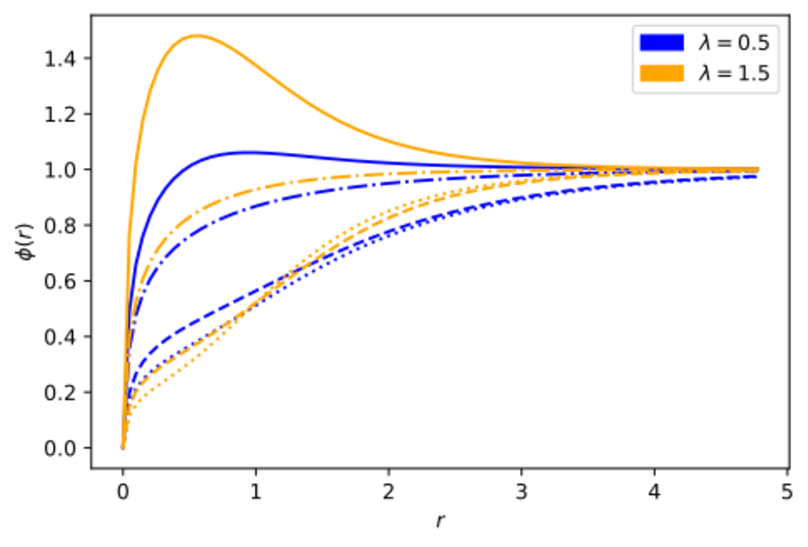
\includegraphics[width = 0.5\textwidth]{gfx/phi_gauss.pdf}}
	\subfloat[Campo de gauge $A_\theta(r)$.]{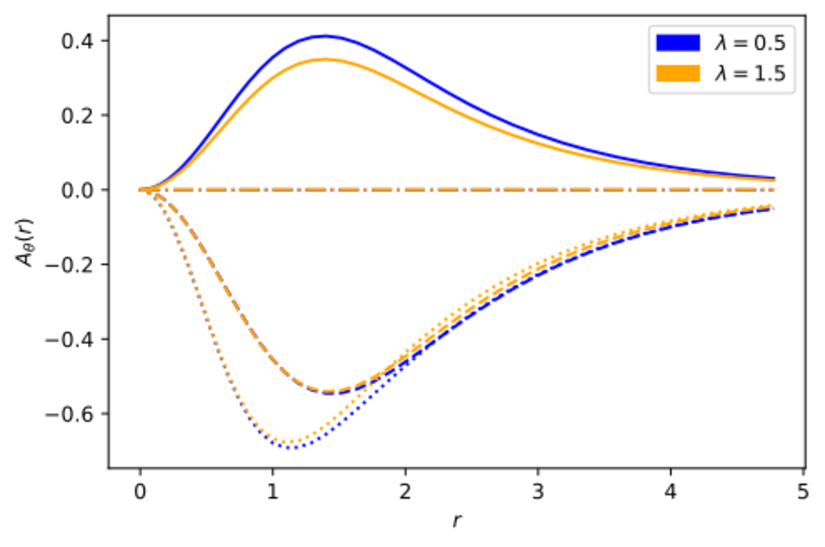
\includegraphics[width = 0.5\textwidth]{gfx/atheta_gauss.pdf}}
	\quad
	\subfloat[Energía de la configuración.]{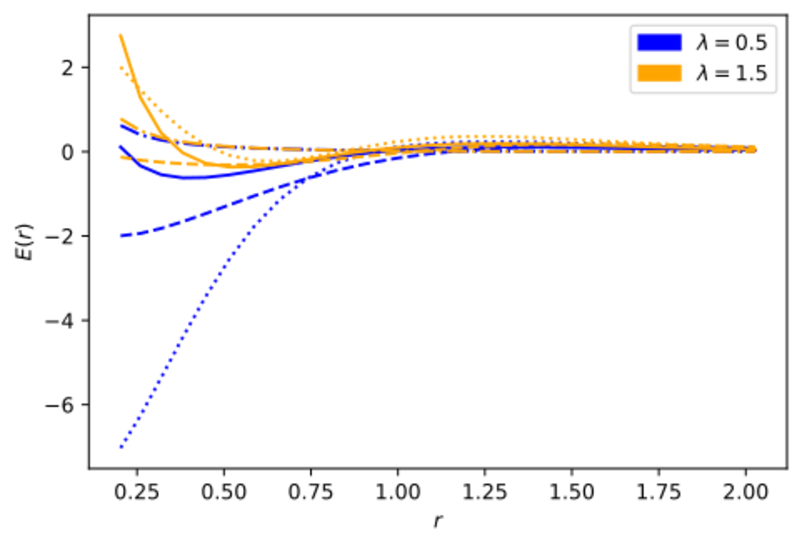
\includegraphics[width = 0.5\textwidth]{gfx/E_gauss.pdf}}
	\subfloat[Campo magnético.]{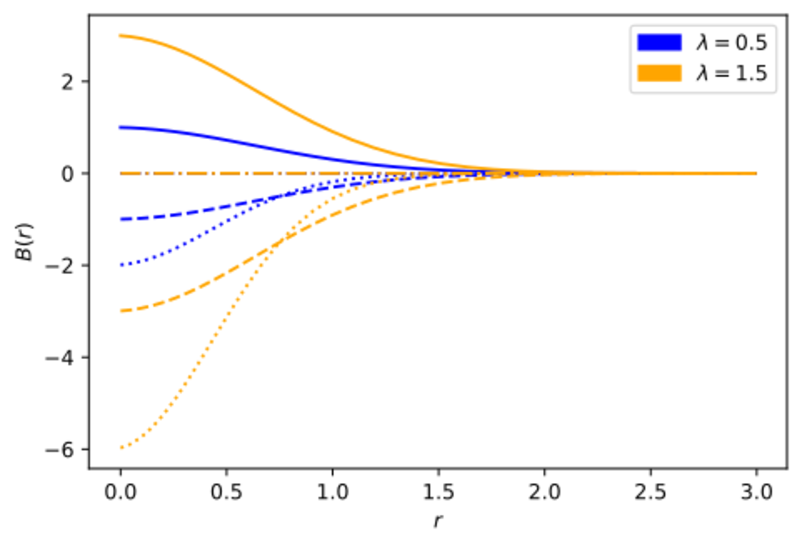
\includegraphics[width = 0.5\textwidth]{gfx/B_gauss.pdf}}
	\caption{Soluciones de vacío obtenidas minimizando numéricamente el potencial \eqref{eq:7.4.0.1}. Se muestra en azul las soluciones con $\lambda = 0.5$ y en naranja con $\lambda = 1.5$. Además, se muestran soluciones para distintas impurezas, a saber: $\sigma(r)=4 e^{-r^2}$ en líneas sólidas, $\sigma(r) = -4e^{-r^2}$ en líneas discontinuas y $\sg(r)=-8e^{-2r^2}$ en líneas punteadas. Como adicional, también se muestra las solución de vacío sin impurezas en líneas punteadas y discontinuas.}
	\label{fig:field_gauss}
\end{figure}

\begin{figure}[t]
	\centering
	\subfloat[Perfil del campo $\phi(r)$.]{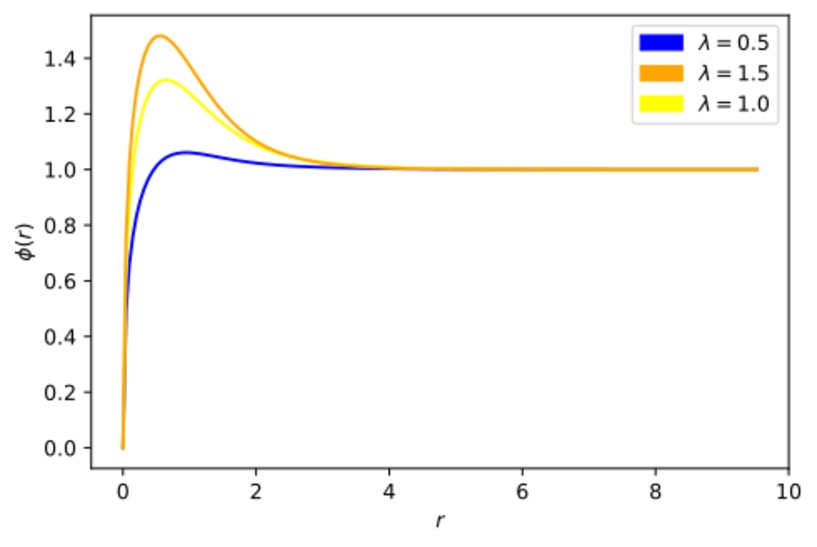
\includegraphics[width = 0.5\textwidth]{gfx/phi_lambdas.pdf}}
	\subfloat[Campo de gauge $A_\theta(r)$.]{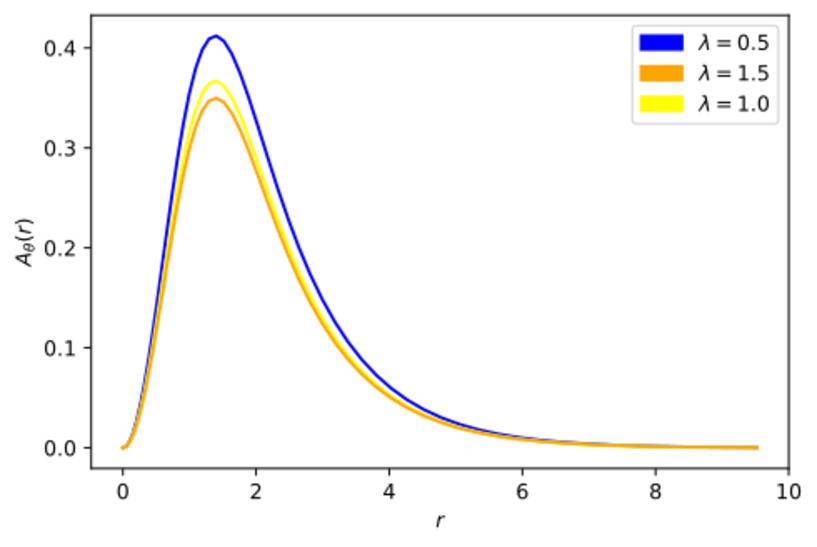
\includegraphics[width = 0.5\textwidth]{gfx/atheta_lambdas.pdf}}
	\quad
	\subfloat[Energía de la configuración.]{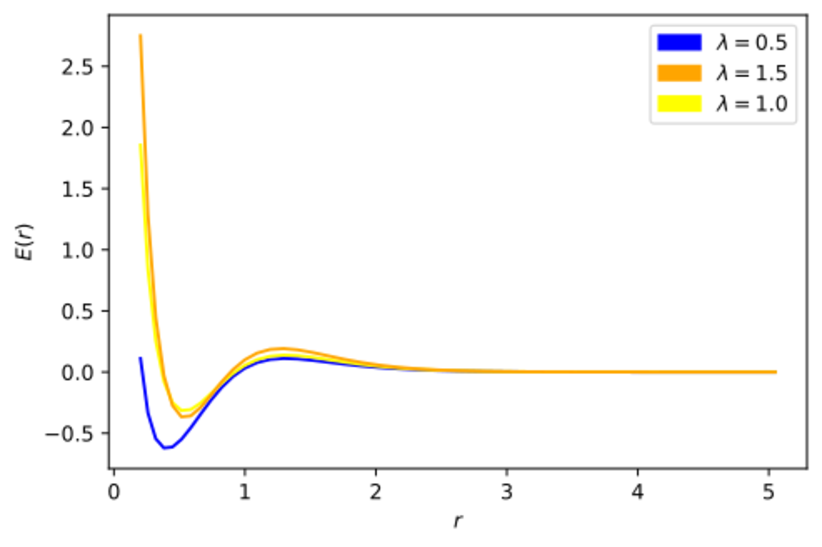
\includegraphics[width = 0.5\textwidth]{gfx/E_lambdas.pdf}}
	\subfloat[Campo magnético.]{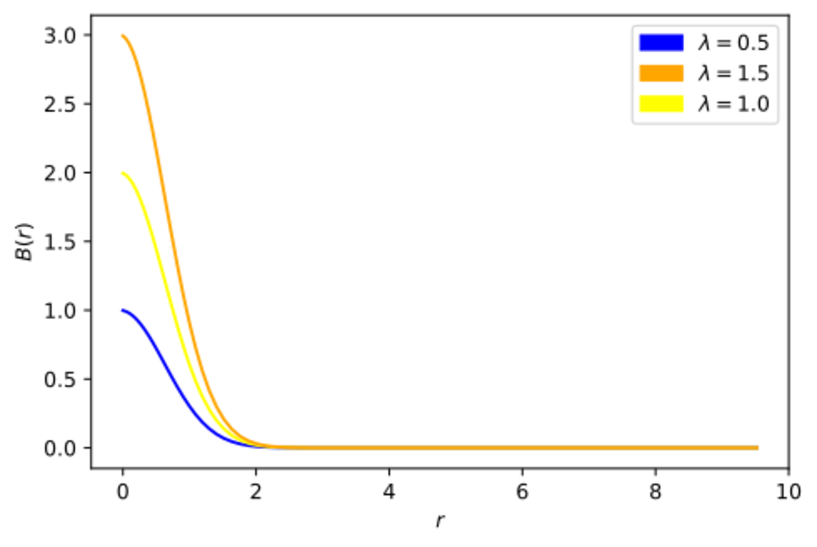
\includegraphics[width = 0.5\textwidth]{gfx/B_lambdas.pdf}}
	\caption{Soluciones de vacío obtenidas minimizando numéricamente el potencial \eqref{eq:7.4.0.1}. Se muestran soluciones para tres valores distintos de $\lambda$ en presencia de la impureza $\sg(r)=4e^{-r^2}$.}
	\label{fig:field_lambdas}
\end{figure}


 % Chapter 3
%% Chapter X

\chapter{Chapter Title} % Chapter title

\label{ch:name} % For referencing the chapter elsewhere, use \autoref{ch:name} 

%----------------------------------------------------------------------------------------

\section{Section Title}

Content

%------------------------------------------------

\subsection{Subsection Title}

Content

%------------------------------------------------

\subsection{Subsection Title}

Content

%----------------------------------------------------------------------------------------

\section{Section Title}

Content % Chapter 4 - empty template

\cleardoublepage % Empty page before the start of the next part

% Conclusiones

\chapter{Conclusiones y posible futuro trabajo}

\label{ch:conclusiones}

Este trabajo presenta un estudio bastante amplio sobre vórtices en el modelo Abeliano de Higgs. En el primer capítulo estudiamos lo básico sobre vórtices en el espacio plano.

%----------------------------------------------------------------------------------------
%	THESIS CONTENT - APPENDICES
%----------------------------------------------------------------------------------------

\appendix

\part{Apéndices} % New part of the thesis for the appendix

% Appendix A

\chapter{Appendix Test}

%----------------------------------------------------------------------------------------

\lipsum[13-14]

%----------------------------------------------------------------------------------------

\section{Appendix Section Test}
\lipsum[15]

\graffito{More dummy text}
\lipsum[16]

%----------------------------------------------------------------------------------------

\section{Another Appendix Section Test}
\lipsum[17]

\begin{table}
\myfloatalign
\begin{tabularx}{\textwidth}{Xll} \toprule
\tableheadline{labitur bonorum pri no} & \tableheadline{que vista}
& \tableheadline{human} \\ \midrule
fastidii ea ius & germano &  demonstratea \\
suscipit instructior & titulo & personas \\
\midrule
quaestio philosophia & facto & demonstrated \\
\bottomrule
\end{tabularx}
\caption[Autem usu id]{Autem usu id.}
\label{tab:moreexample}
\end{table}

\lipsum[18]

There is also a useless Pascal listing below: \autoref{lst:useless}.

\begin{lstlisting}[float=b,language=Pascal,frame=tb,caption={A floating example (\texttt{listings} manual)},label=lst:useless]
for i:=maxint downto 0 do
begin
{ do nothing }
end;
\end{lstlisting} % Appendix A
%% Appendix X

\chapter{Appendix Title}

%----------------------------------------------------------------------------------------

% Content begins here % Appendix B - empty template

%----------------------------------------------------------------------------------------
%	POST-CONTENT THESIS PAGES
%----------------------------------------------------------------------------------------

\cleardoublepage% Bibliography

\label{app:bibliography} % Reference the bibliography elsewhere with \autoref{app:bibliography}

\manualmark % Work-around to have small caps also here in the headline
\markboth{\spacedlowsmallcaps{\bibname}}{\spacedlowsmallcaps{\bibname}} % Work-around to have small caps also
%\phantomsection
\refstepcounter{dummy}

\addtocontents{toc}{\protect\vspace{\beforebibskip}} % Place the bibliography slightly below the rest of the document content in the table of contents
\addcontentsline{toc}{chapter}{\tocEntry{\bibname}}

\printbibliography % Bibliography
%\cleardoublepage% Declaration

\refstepcounter{dummy}
\pdfbookmark[0]{Declaration}{declaration} % Bookmark name visible in a PDF viewer

\chapter*{Declaration} % Declaration section text

\thispagestyle{empty}

Put your declaration here.
\bigskip
 
\noindent\textit{\myLocation, \myTime}

\smallskip

\begin{flushright}
\begin{tabular}{m{5cm}}
\\ \hline
\centering\myName \\
\end{tabular}
\end{flushright}
 % Declaration

%\cleardoublepage% Colophon (a brief description of publication or production notes relevant to the edition)

\pagestyle{empty}

\hfill

\vfill

\pdfbookmark[0]{Colophon}{colophon}

\section*{Colophon}

This document was typeset using the typographical look-and-feel \texttt{classicthesis} developed by Andr\'e Miede. The style was inspired by Robert Bringhurst's seminal book on typography ``\emph{The Elements of Typographic Style}''. \texttt{classicthesis} is available for both \LaTeX\ and \mLyX: 

\begin{center}
\url{https://bitbucket.org/amiede/classicthesis/}
\end{center}

\noindent Happy users of \texttt{classicthesis} usually send a real postcard to the author, a collection of postcards received so far is featured here: 

\begin{center}
\url{http://postcards.miede.de/}
\end{center}
 
\bigskip
 % Colophon

%----------------------------------------------------------------------------------------

\end{document}
